\documentclass{article}

\usepackage{graphicx}
\usepackage{multirow}
\usepackage{amsmath,amssymb,amsfonts,amsthm, mathrsfs}
\usepackage[title]{appendix}
\usepackage{xcolor}
\usepackage{textcomp}
\usepackage{manyfoot, booktabs}
\usepackage{algorithm, algorithmicx, algpseudocode}
\usepackage{listings}
\usepackage{biblatex}

\usepackage[english]{babel}

\raggedbottom

\lstset{
    language=Python,                 % Especificar el lenguaje
    basicstyle=\ttfamily\small,      % Estilo básico y tamaño de fuente
    keywordstyle=\color{blue},       % Estilo para las palabras clave
    stringstyle=\color{red},         % Estilo para las cadenas de texto
    commentstyle=\color{orange},      % Estilo para los comentarios
    morecomment=[s][\color{gray}]{"""}{"""}, % Estilo para comentarios multilínea
    numbers=left,                    % Números de línea a la izquierda
    numberstyle=\tiny\color{gray},   % Estilo de los números de línea
    stepnumber=1,                    % Distancia entre números de línea
    numbersep=10pt,                  % Separación entre código y números de línea
    backgroundcolor=\color{white},   % Color de fondo
    showspaces=false,                % No mostrar espacios
    showstringspaces=false,          % No mostrar espacios en cadenas de texto
    showtabs=false,                  % No mostrar tabs
    frame=single,                    % Marco simple alrededor del código
    captionpos=b,                    % Posición de la leyenda (bottom)
    breaklines=true,                 % Romper líneas largas
    breakatwhitespace=false,         % Romper líneas solo en espacios
    tabsize=4,                       % Tamaño del tabulador
    escapeinside={\%*}{*)}           % Permitir LaTeX dentro del código
}

\begin{document}

\title{F1 EDA: Hadoop Cluster with Hive: Big Data 2nd Term}

\author{Enrique Ulises Báez Gómez Tagle \\ Mauricio Iván Ascencio Martínez\\ Sara Rocío Miranda Mateos}

\maketitle

\begin{abstract}
This project focuses on constructing a Hadoop cluster integrated with a Hive database to conduct exploratory data analysis (EDA) on Formula 1 dataset. Our objective is to leverage big data technologies to uncover insights into F1 races, drivers, and performance metrics. The document outlines the technological infrastructure setup, data analysis methodology, key findings, encountered challenges, and the solutions we implemented.
\end{abstract}

\tableofcontents
\newpage

\section{Introduction}
In the fast-paced world of Formula 1 racing, where milliseconds can determine the winner, the application of big data technologies opens up new vistas for understanding and optimizing performance. This project embarks on an exploratory journey into the vast datasets of Formula 1 races, employing Hadoop and Hive to manage and analyze this data. The goal is not only to illustrate the capabilities of these technologies in handling large-scale data, but also to explore how big data can provide unprecedented insights into race strategies, driver efficiency, and team dynamics. Our exploration goes beyond traditional analytics, delving into the nuances of data-driven decision-making in sports. Through this document, we aim to share our journey from the initial setup of our big data infrastructure to the nuanced analysis that led us to compelling insights and the myriad challenges we navigated along the way.

\section{Infrastructure / Architecture}
The foundation of our data analysis project is a meticulously designed Hadoop cluster, augmented with Hive to facilitate structured data storage and sophisticated querying capabilities. Our infrastructure not only ensures the efficient handling of big data but also supports complex exploratory data analysis (EDA) processes. The architecture is strategically deployed on the Google Cloud Platform (GCP), leveraging its scalable compute and storage services. Below is a comprehensive outline of our deployment strategy:

\begin{itemize}
    \item \textbf{Hadoop Cluster Configuration:} Central to our project is a Hadoop cluster, designed for scalability and resilience. We configured it with one master node to manage the cluster and multiple worker nodes to process the data. This setup allows for efficient data processing and analysis.
    
    \item \textbf{Hive Database Integration:} For querying capabilities, we integrated Hive with our Hadoop cluster. Hive facilitates querying and managing large datasets residing in distributed storage using SQL-like syntax. It is particularly advantageous for EDA, allowing us to query the data stored in the Hadoop Distributed File System (HDFS) with ease.
    
    \item \textbf{MySQL Cloud SQL Instance for Hive Metastore:} The metadata for Hive tables, such as schema information, is managed by a MySQL instance hosted on Cloud SQL. This setup ensures that the metadata is stored reliably and is accessible across the cluster, enabling efficient query processing.
    
    \item \textbf{Cloud Storage for Hive Warehouse:} The processed and raw data are stored in a Cloud Storage bucket designated as the Hive Warehouse. This choice of storage solution offers high availability and scalability, essential for managing the large datasets involved in our project.
    
    \item \textbf{Deployment Process:}
        \begin{enumerate}
            \item We initiated our deployment by setting up the Google Cloud SDK, enabling us to interact with Google Cloud services seamlessly.
            \item A Cloud Storage bucket was created to host our Hive data, carefully chosen to be in proximity to our compute resources to minimize latency.
            \item We proceeded to establish a Cloud SQL instance for MySQL, tailored to serve as the Hive Metastore. This instance was configured with recommended settings to balance performance with cost efficiency.
            \item The creation of the Dataproc Cluster was a pivotal step, involving the activation of the Cloud Dataproc API and the configuration of the cluster to suit our processing needs. We opted for a standard cluster with a specific mix of master and worker nodes, ensuring adequate resources for our data processing tasks.
            \item Service accounts were configured with precise permissions to manage resources across Cloud SQL and Dataproc, streamlining the interaction between different components of our architecture.
        \end{enumerate}
\end{itemize}

This infrastructure serves as the backbone for our project, enabling us to leverage big data technologies effectively to extract meaningful insights from the Formula 1 dataset. The deployment emphasizes scalability, efficiency, and cost-effectiveness, tailored to meet the demands of processing and analyzing large-scale data.

\begin{figure}[H]
    \centering
    \includegraphics[width=0.9\textwidth]{diagram-arch.png}
    \caption{\textbf{Architecture Diagram}}
\end{figure}

\section{Data Analysis with F1 Dataset}
In our exploration of big data applications within Formula 1 racing, we obtained a dataset from Kaggle, which encompasses detailed information about the 2023 Formula 1 season. The dataset can be found at \url{https://www.kaggle.com/datasets/juampimgi/formula-1-season-2023?resource=download}. This dataset includes valuable data on race results, driver standings, lap times, and much more, providing a rich basis for our exploratory data analysis (EDA).

Our analysis focused on extracting actionable insights that could potentially influence race strategies and improve team and driver performances. To achieve this, we executed several Hive SQL queries on our Hadoop cluster to handle the large volumes of data efficiently. Each query was designed to test specific hypotheses about correlations between different variables such as weather conditions, circuit characteristics, and driver performance metrics. After obtaining preliminary results from these queries and formulating initial conclusions, we enhanced our analysis, by exporting these results to CSV files, which were then used for creating detailed visualizations in R. This additional step enabled us to achieve a more visual and intuitive understanding of the data, simplifying the derivation of valuable conclusions from the patterns observed in the results.

\subsection{Database Structure Overview}
For our exploratory data analysis (EDA), we used a dataset from the 2023 season, which is structured into several tables with specific focuses. Each table captures unique aspects of the sport, allowing for a comprehensive analysis from multiple angles. Here's a brief guide to the tables:

\begin{itemize}
    \item \textbf{Events}: Contains information about each race event, including location, dates, and session details.
    \item \textbf{Fastest Laps}: Records the fastest lap times achieved during a race, along with related performance metrics.
    \item \textbf{Laps}: Details every lap completed during the race weekends, with timing and telemetry data.
    \item \textbf{Results}: Summarizes race results, positions, and points for drivers and teams.
    \item \textbf{Sprint Laps}: Focuses on the laps during sprint qualifying sessions, a shorter race format that determines starting positions.
    \item \textbf{Sprint Results}: Outlines the outcomes of sprint qualifying sessions, including grid positions and points.
    \item \textbf{Telemetry}: Provides technical data such as speed, gear, and throttle usage throughout the laps.
    \item \textbf{Weather}: Captures the weather conditions at the event location, which can significantly impact race dynamics.
\end{itemize}

\subsection{Query Execution Framework}

To conduct our analysis, we utilized a Spark SQL query execution framework that allowed us to maintain a consistent approach across most of our queries. The majority of queries were executed using a standard template in Spark, which we adapted for specific needs when necessary. This template ensured that all queries were run efficiently and reliably within the Spark environment with Hive support enabled.

The following code snippet outlines the general structure used to execute our SQL queries:

\begin{lstlisting}[language=Python]
from pyspark.sql import SparkSession

# Initialize a SparkSession with Hive support enabled
spark = SparkSession.builder
    .appName("SQL Query Template")
    .enableHiveSupport()
    .getOrCreate()

# Define SQL Query
sql_query = """
"""

# Execute the SQL query
result_df = spark.sql(sql_query)

# Display the results to verify them
result_df.show()

# Stop the Spark session to free up resources when done
spark.stop()
\end{lstlisting}

\subsection{Query Analysis and Insights}

\subsubsection{Average Number of Laps per Grand Prix}
\paragraph{Description:}
This query aims to determine the average number of laps completed in each Grand Prix event. The analysis provides insights into race durations and can help identify tracks with higher or lower average laps, potentially influencing race strategy.

\begin{figure}[H]
    \centering
    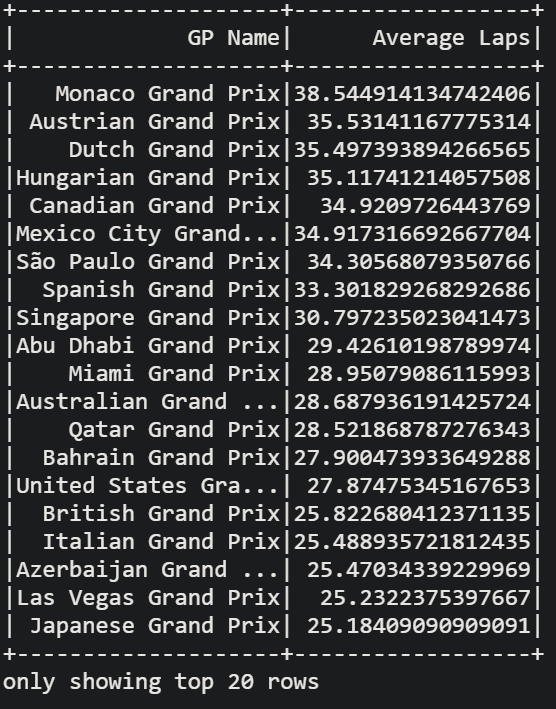
\includegraphics[width=0.6\textwidth]{ss-average-laps.png}
    \caption{Number of Laps GCP Querie Result}
\end{figure}

\begin{figure}[H]
    \centering
    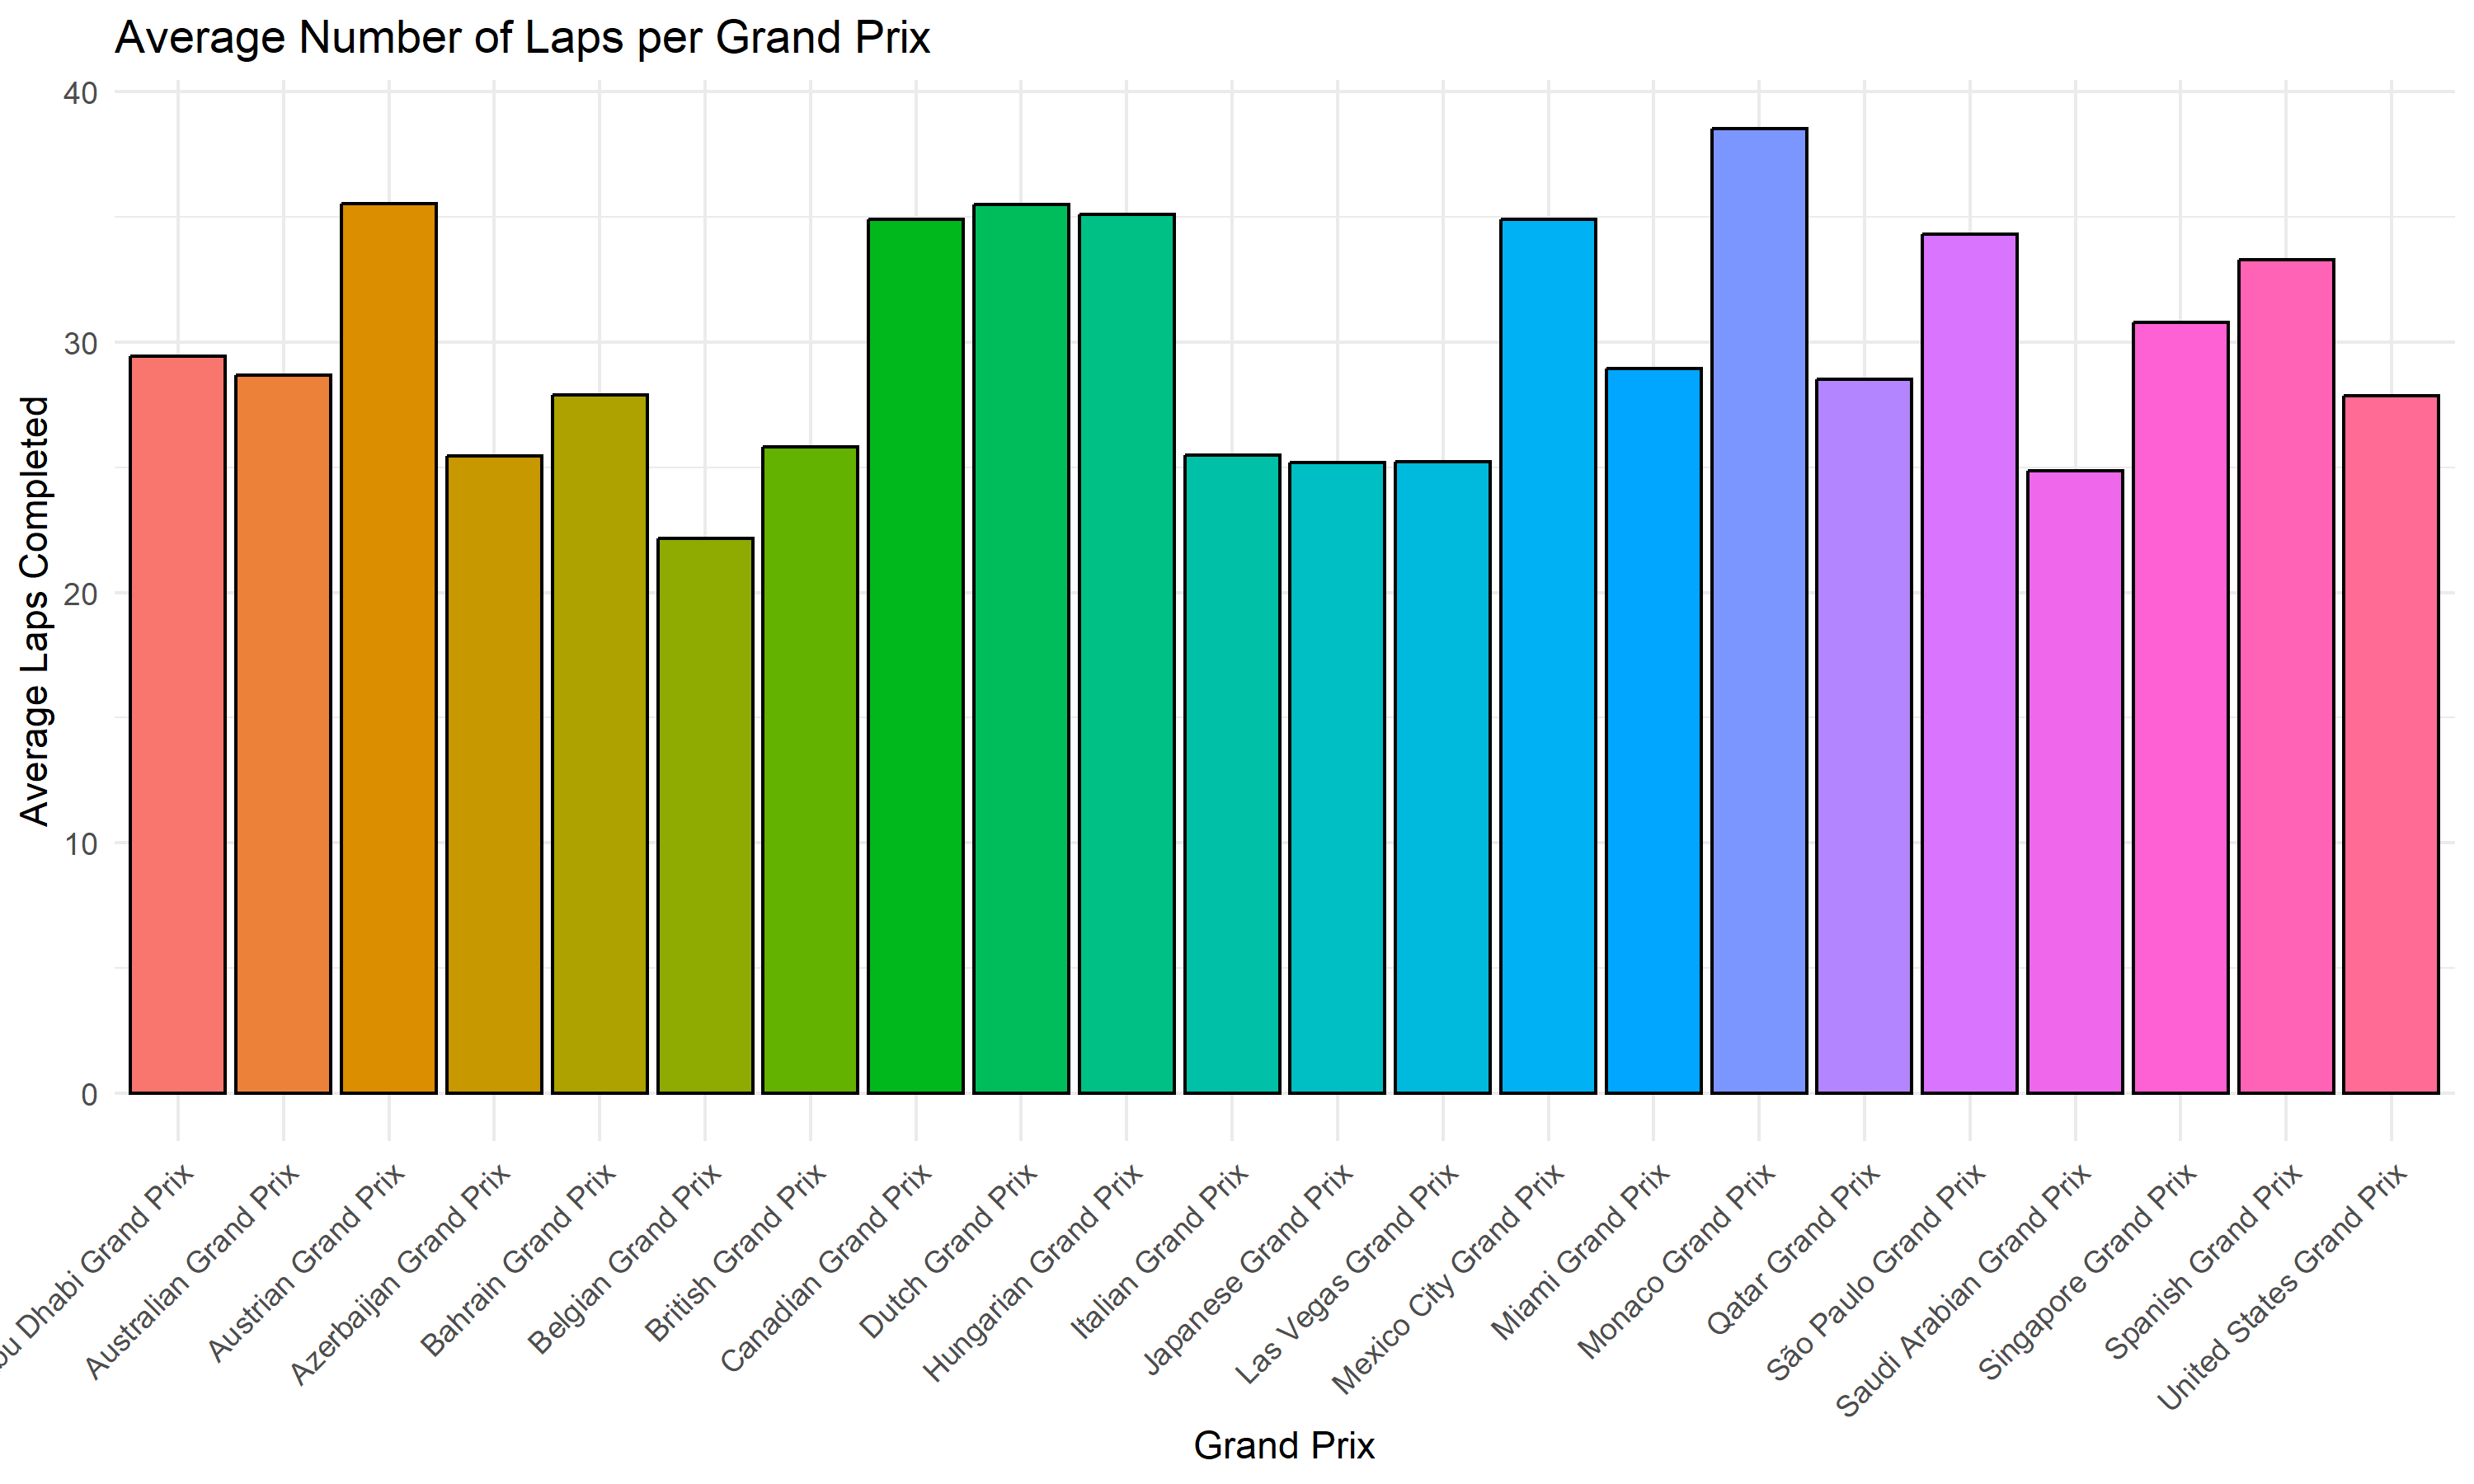
\includegraphics[width=\textwidth]{average_laps_per_gp_plot.png}
    \caption{Bar Chart Average Number of Laps per Grand Prix}
\end{figure}

\paragraph{Interpretation:}
The bar graph visually represents the average number of laps for each Grand Prix, sorted in descending order. Longer races may indicate a need for different tire strategies or fuel management plans. Conversely, shorter races might lead to more aggressive racing tactics. We can say that Monaco GP is the longest and Belgian GP is the shortest with a difference of around 16 laps.


\subsubsection{Average Speed per Sector}
\paragraph{Description:}
This query calculates the average speed for each sector across all laps where speed data is available. It helps in understanding which sectors of the track might demand higher technical skills or allow for greater speeds.

\begin{figure}[H]
    \centering
    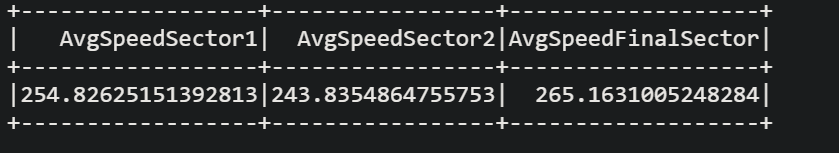
\includegraphics[width=\textwidth]{average-speed-sector.png}
    \caption{Speed Per Sector GCP Querie Result}
\end{figure}

\begin{figure}[H]
    \centering
    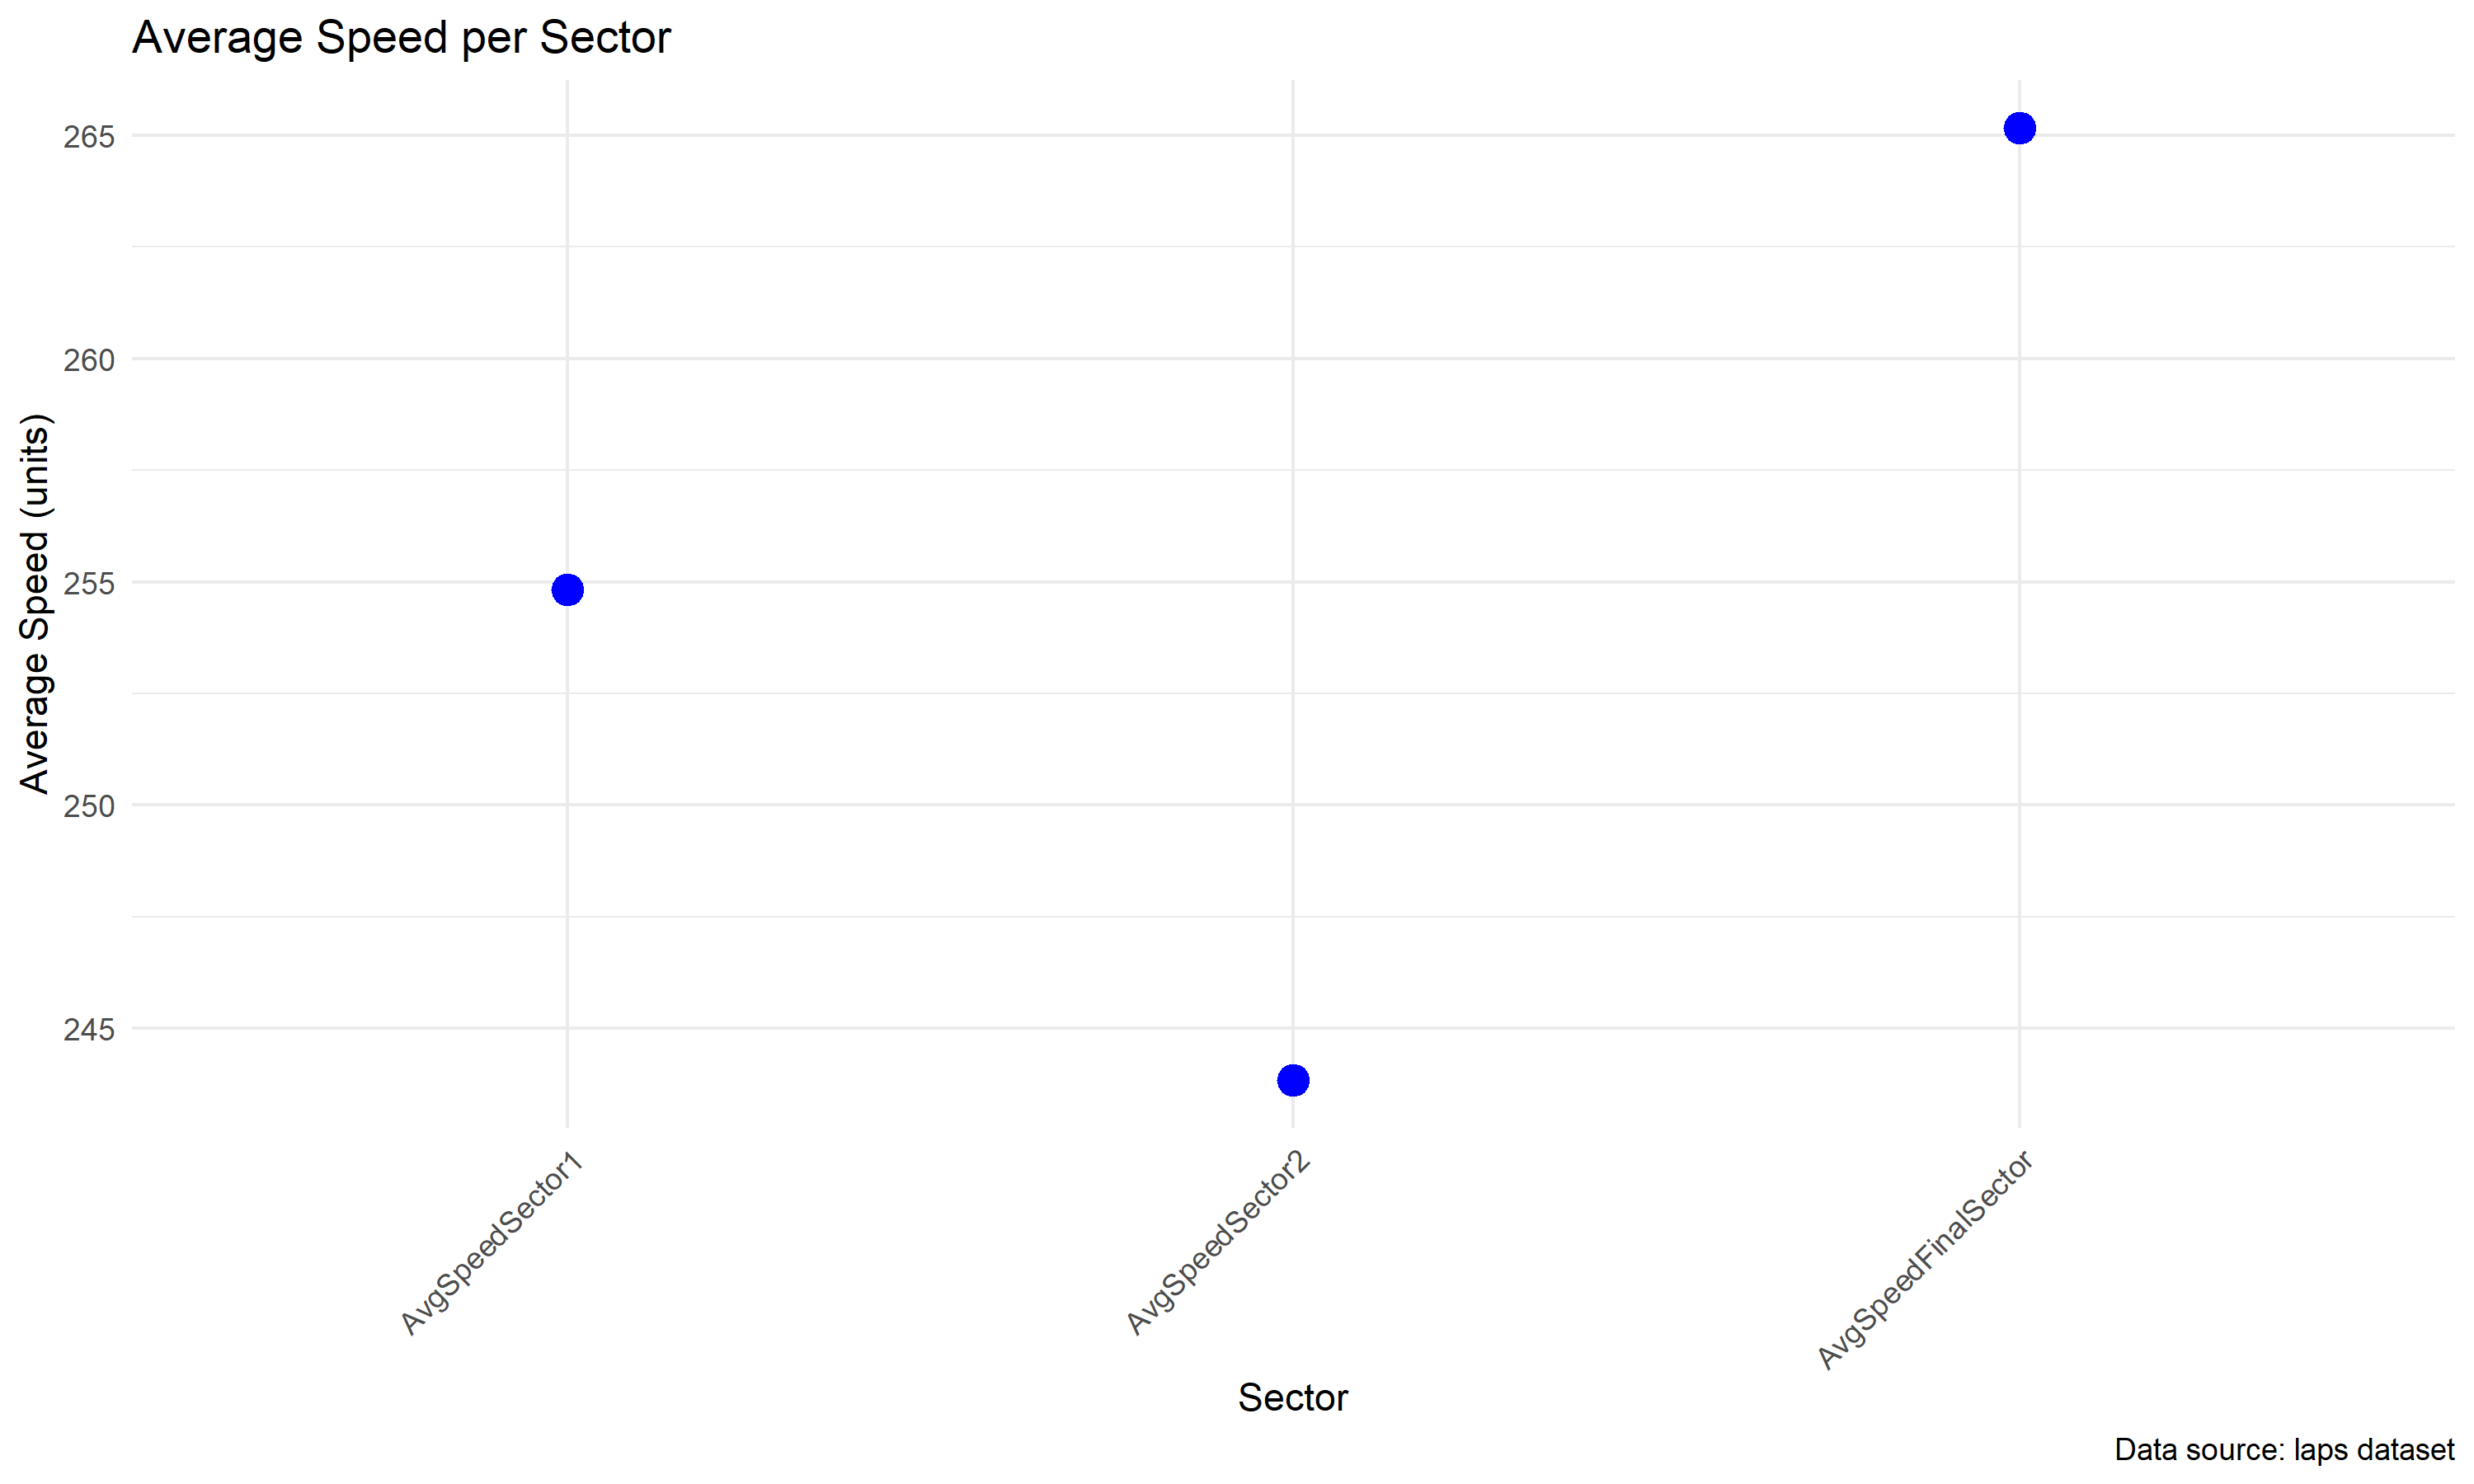
\includegraphics[width=\textwidth]{average_speeds_per_sector_plot.png}
    \caption{Scatter Plot: Average Speed per Sector}
\end{figure}

\paragraph{Interpretation:}
The scatter plot displays the average speeds for the first, second, and final sectors. From this, we can interpret that the final sector allows for higher speeds, which could be crucial for overtaking or qualifying laps. Conversely, the first and second sectors show lower speeds, possibly indicating tighter corners or technical parts of the track where drivers must balance speed with precision.

\subsubsection{Best Lap Times per Grand Prix}
\paragraph{Description:}
This query identifies the best lap time achieved for each Grand Prix. It gives us a benchmark to aim for when seeking to achieve a fast lap time. Notably, a modification was made to this query to use a later-described data integrity check, ensuring accurate differentiation between null values and empty strings. The full process of this data verification will be outlined later.

\begin{figure}[H]
    \centering
    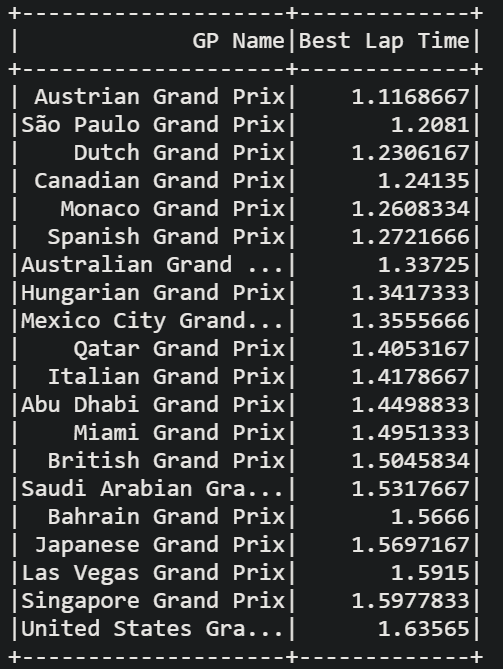
\includegraphics[width=0.6\textwidth]{bestt-lap-times.png}
    \caption{Best Lap Times per Grand Prix GCP Querie Result}
\end{figure}

\begin{figure}[H]
    \centering
    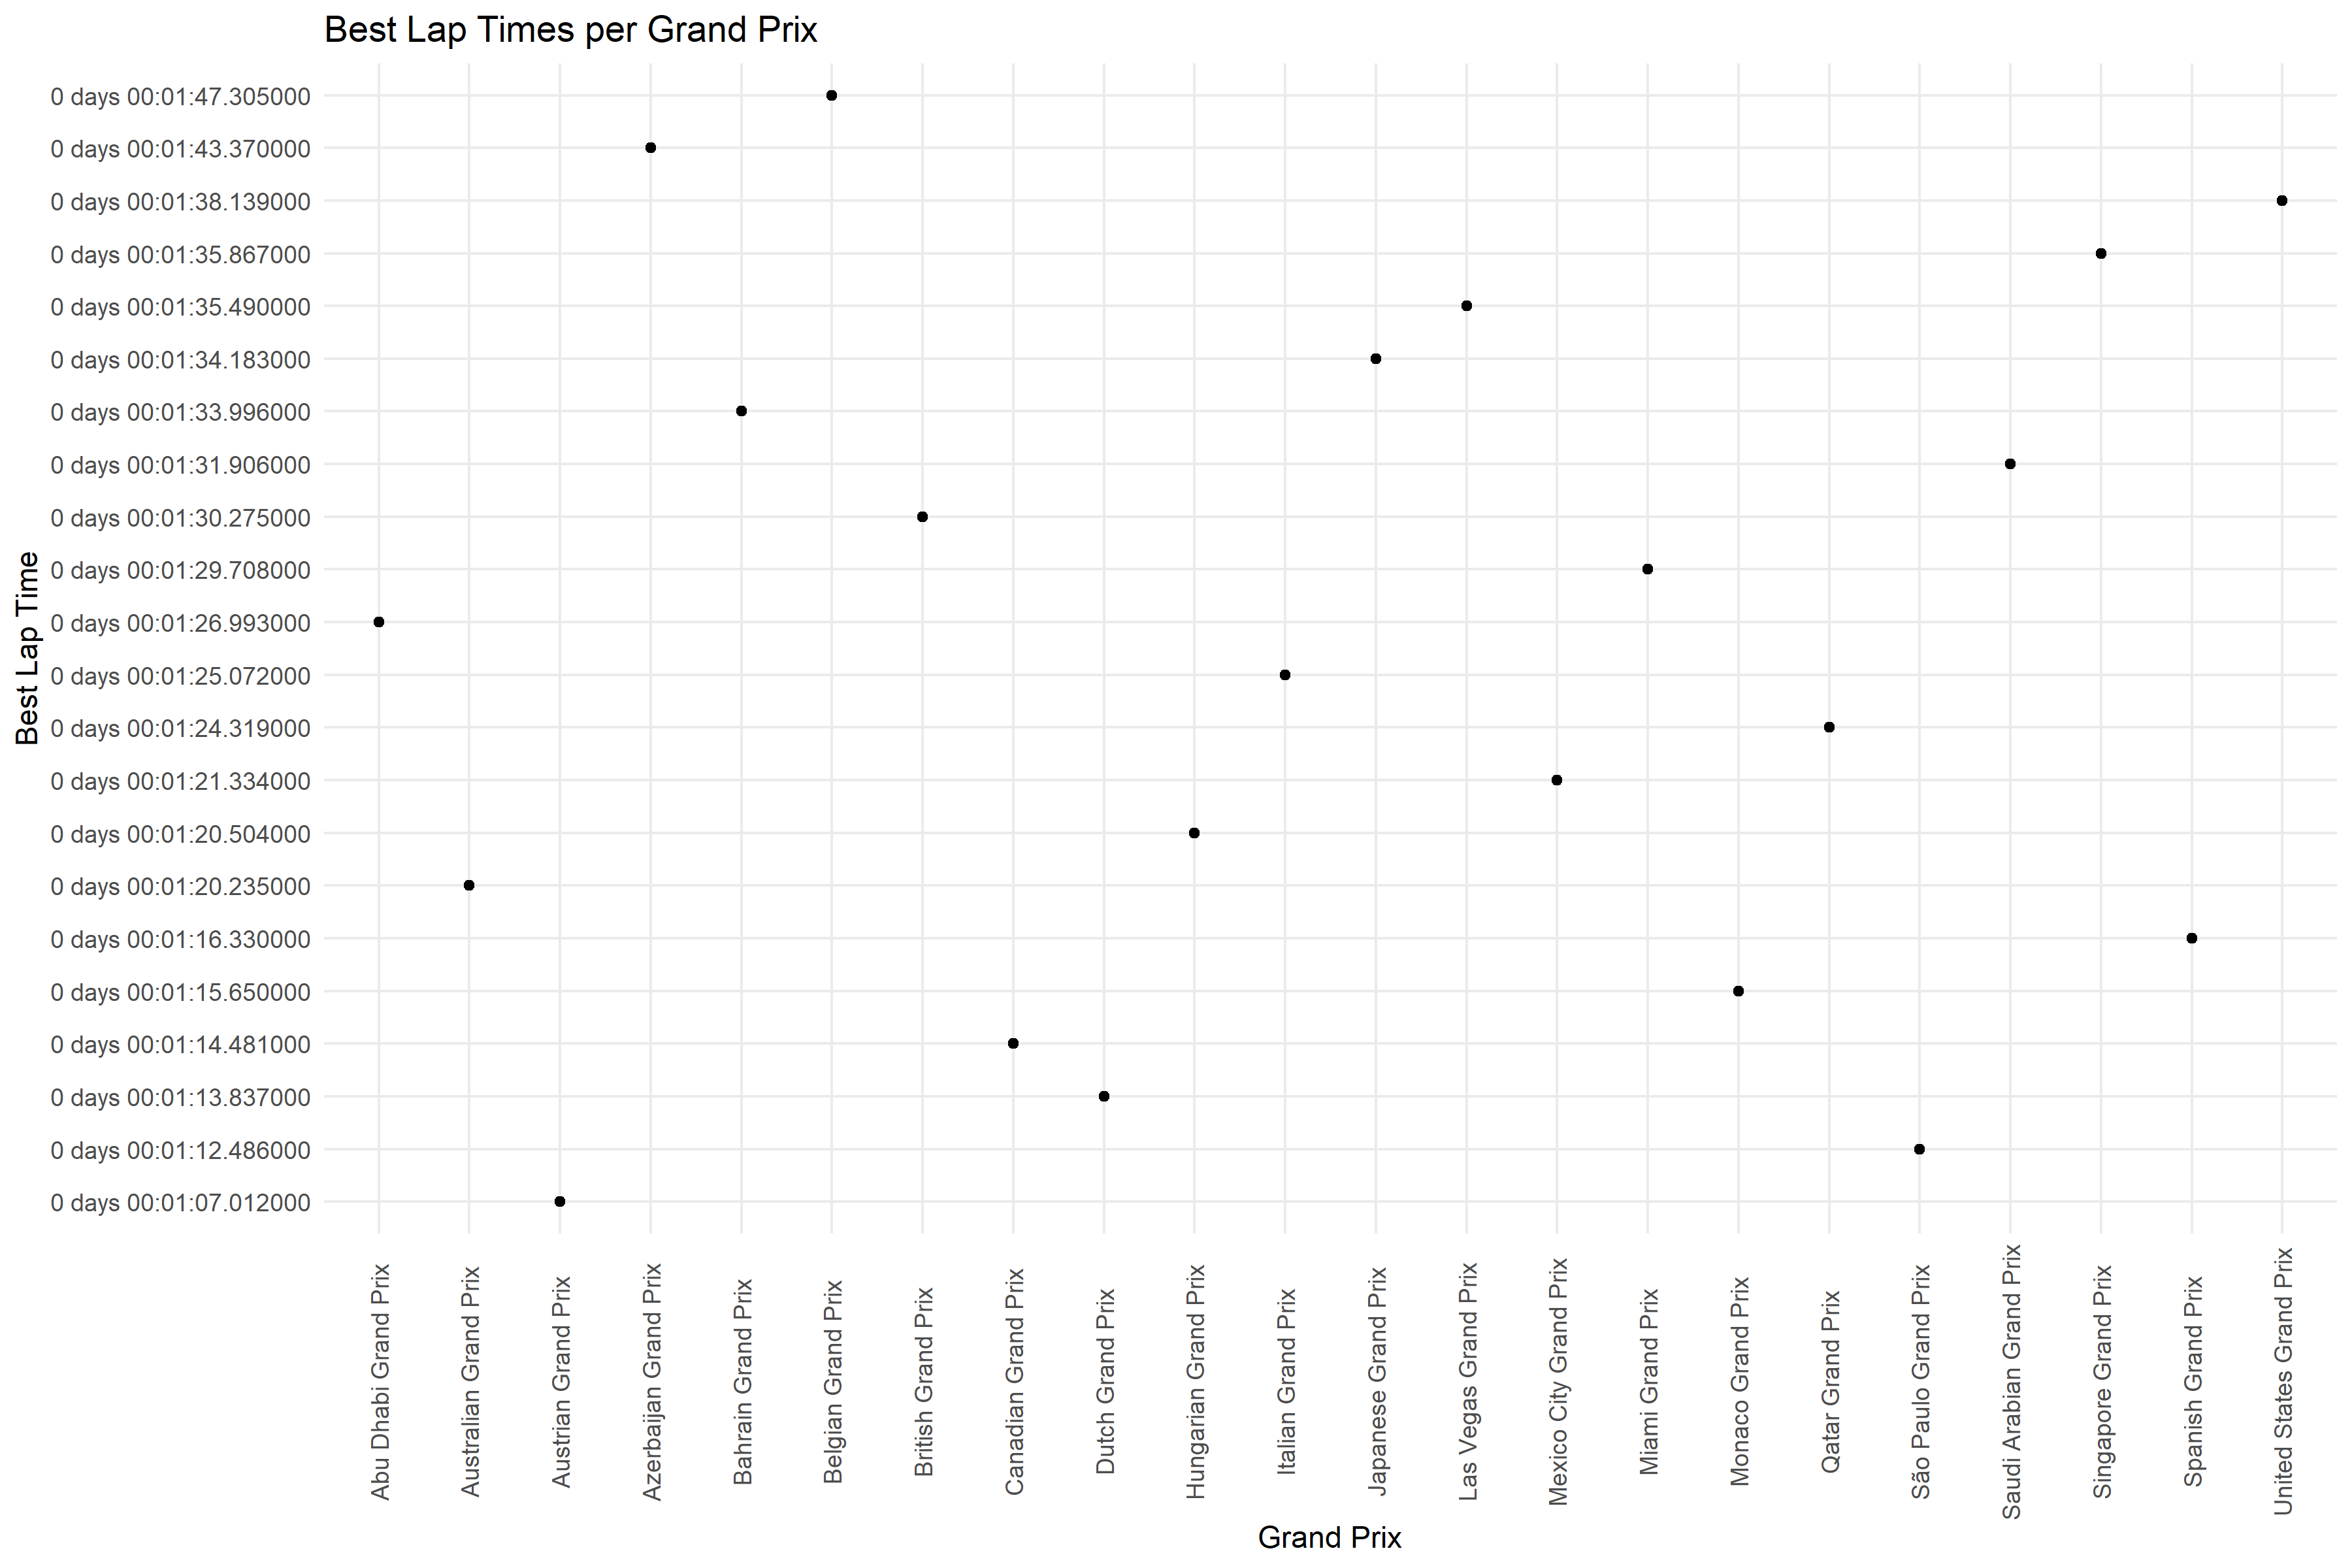
\includegraphics[width=\textwidth]{best_lap_times_per_gp_dotplot.png}
    \caption{Dot plot of the Best Lap Times per Grand Prix visualized using R}
\end{figure}

\paragraph{Interpretation:}
The dot plot illustrates the best lap times for each Grand Prix, highlighting the disparity in circuit performance. It's interesting to see how, even in small increments, there are significant variations in lap times across different Grand Prix events. This underscores the importance of analyzing circuit performance, as even minor differences can impact race outcomes.

\subsubsection{Density of Number of Drivers in Grand Prix Events}
\paragraph{Description:}
This query assesses the frequency at which the starting grid is at full capacity by counting the distinct number of drivers in each Grand Prix event. This metric highlights the Grand Prix events where the grid was complete, providing insights into participation consistency which may impact the overall competitiveness and race dynamics.


\begin{figure}[H]
    \centering
    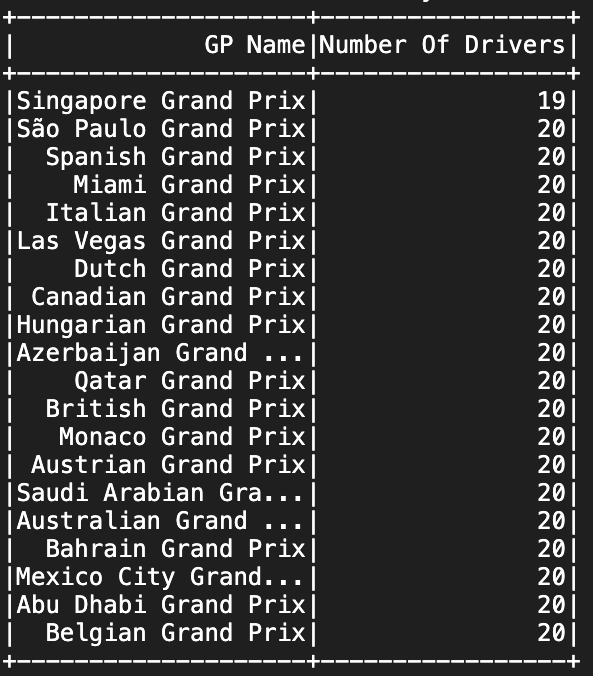
\includegraphics[width=0.5\textwidth]{ss-driver-num.png}
    \caption{Density Number of Drivers GCP Querie Result}
\end{figure}

\begin{figure}[H]
    \centering
    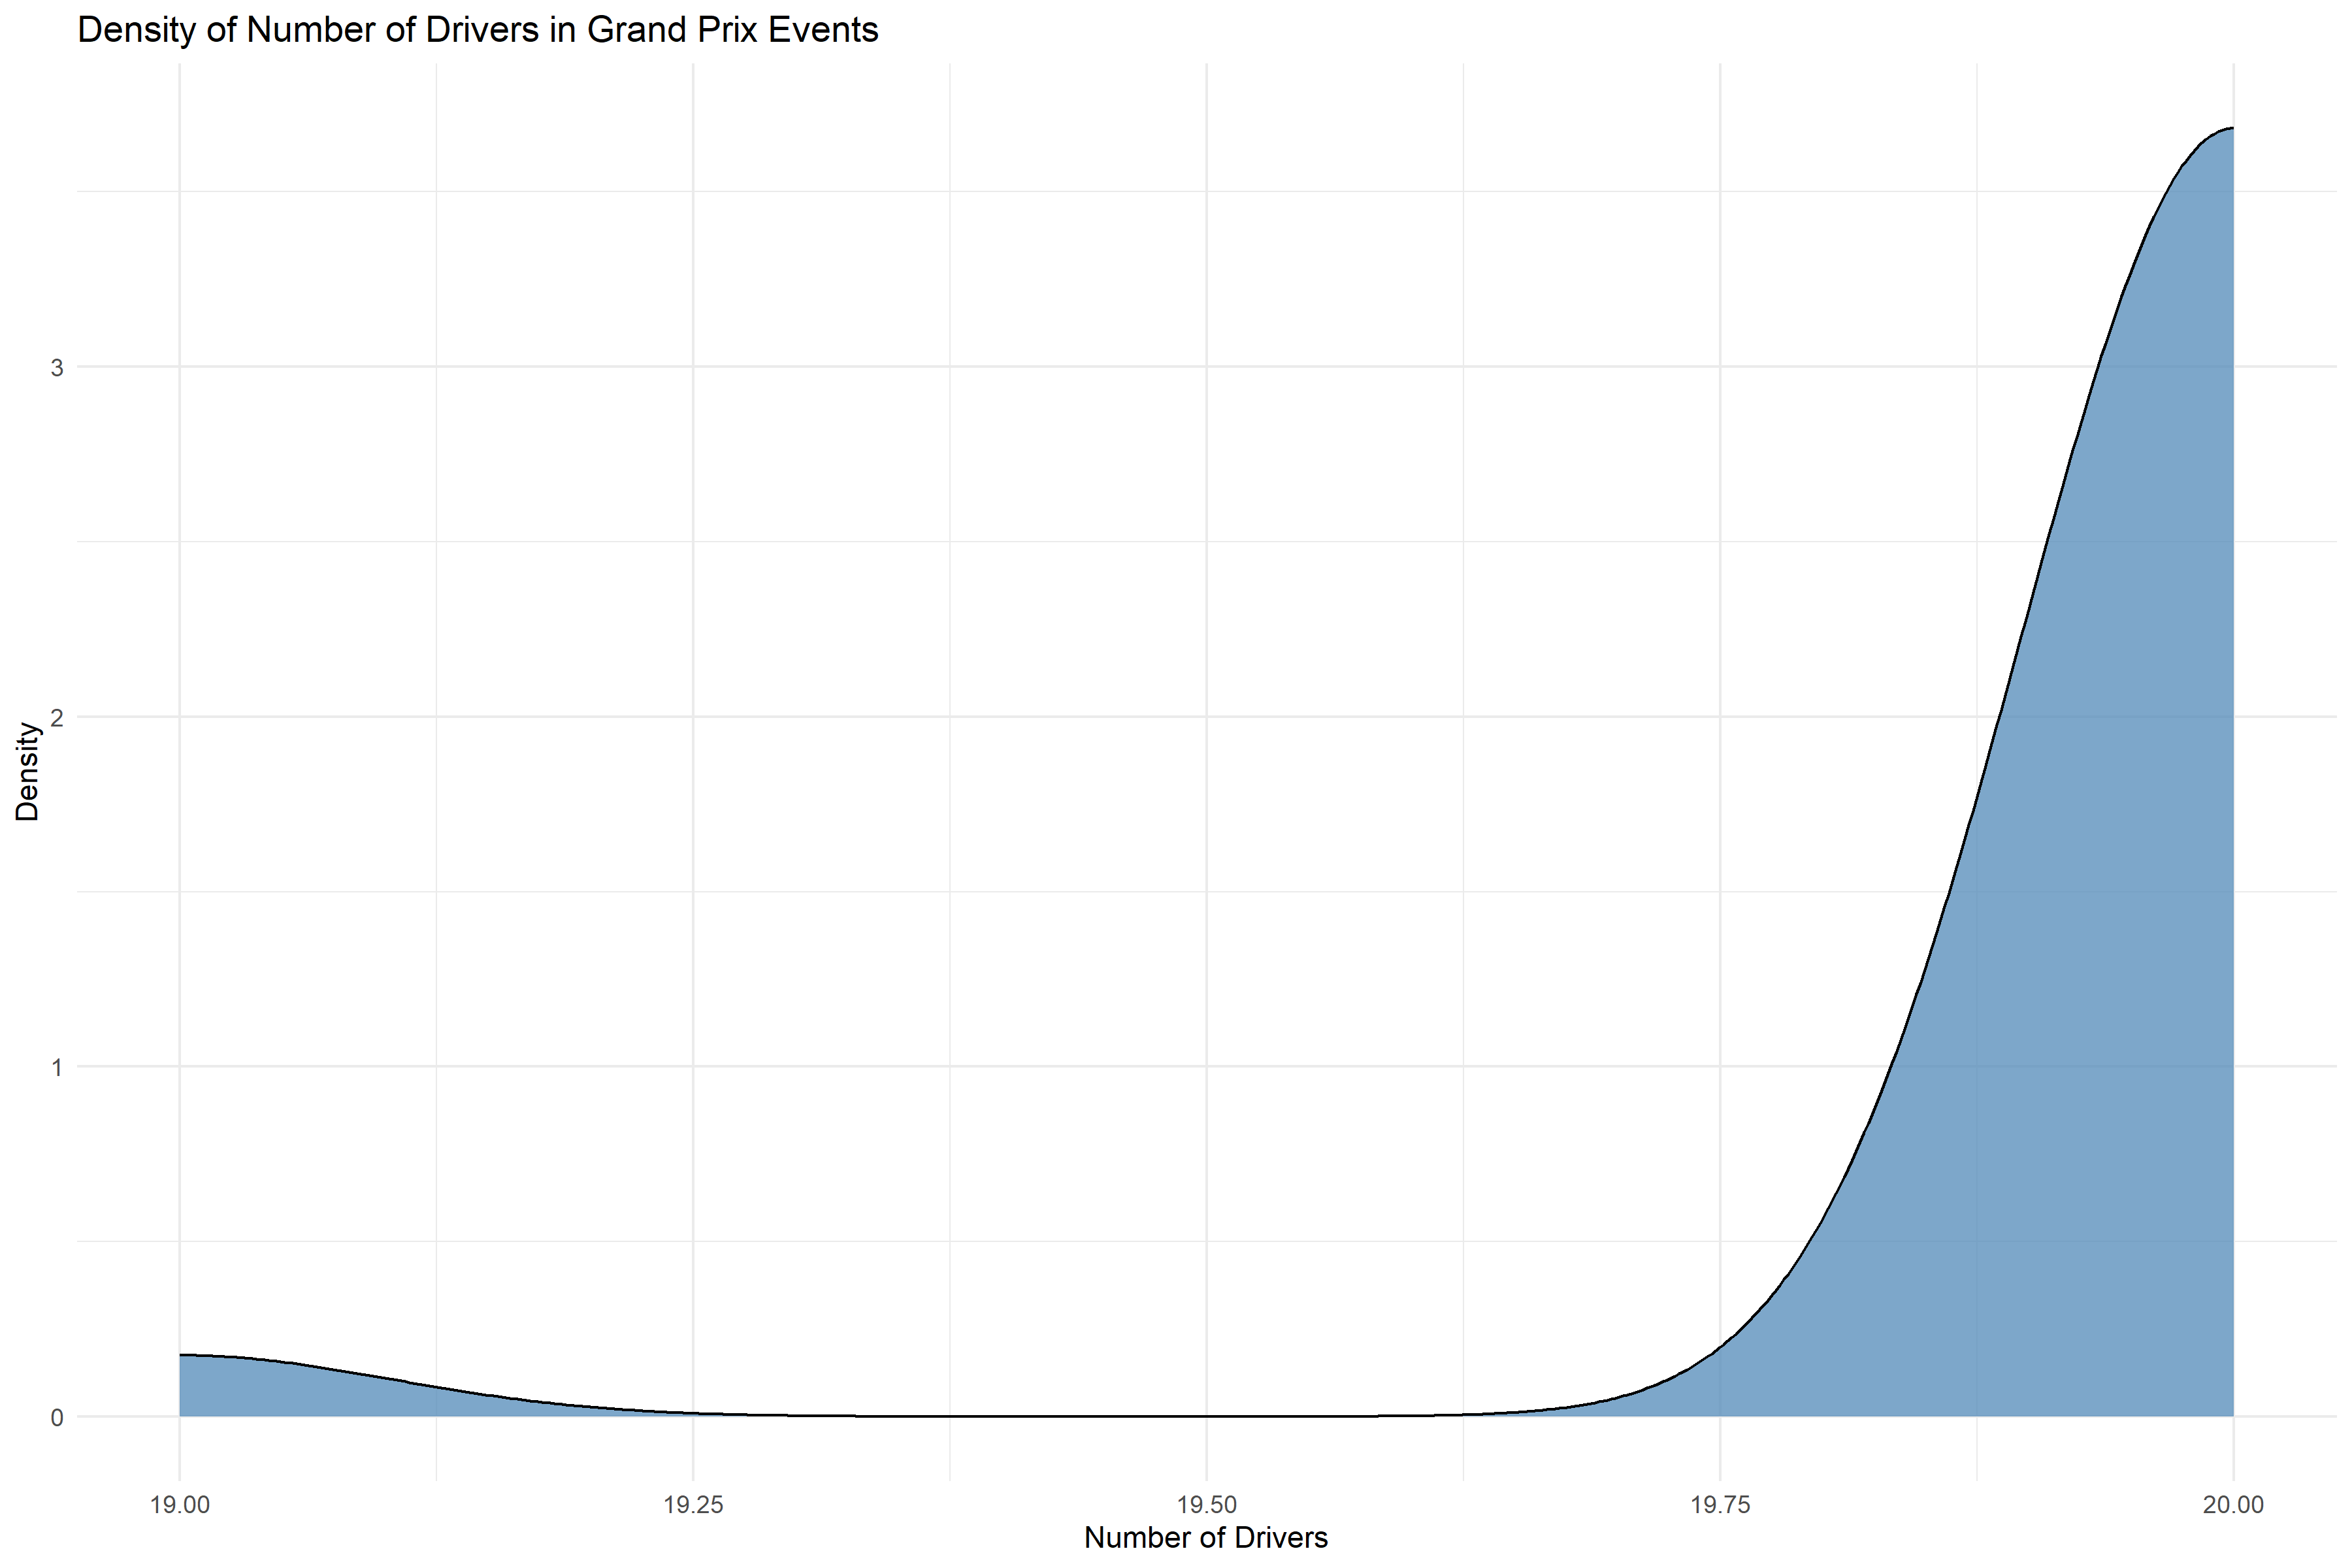
\includegraphics[width=\textwidth]{drivers_density.png}
    \caption{Density Plot of the Number of Drivers per Grand Prix}
\end{figure}

\paragraph{Interpretation:}
The density plot provides a visual distribution of the number of distinct drivers participating in each Grand Prix event. It helps to identify the general trend in driver participation across the season. This analysis can be particularly useful for teams and organizers in understanding the draw of each event and planning strategies.

\subsubsection{Grand Prix Schedule 2023}
\paragraph{Description:}
This query lists all the events in the 2023 Formula 1 season, sorted by date. It helps to visualize the distribution of Grand Prix events throughout the year, providing insight into the periods with the most intense schedules for the teams and drivers.

\begin{figure}[H]
    \centering
    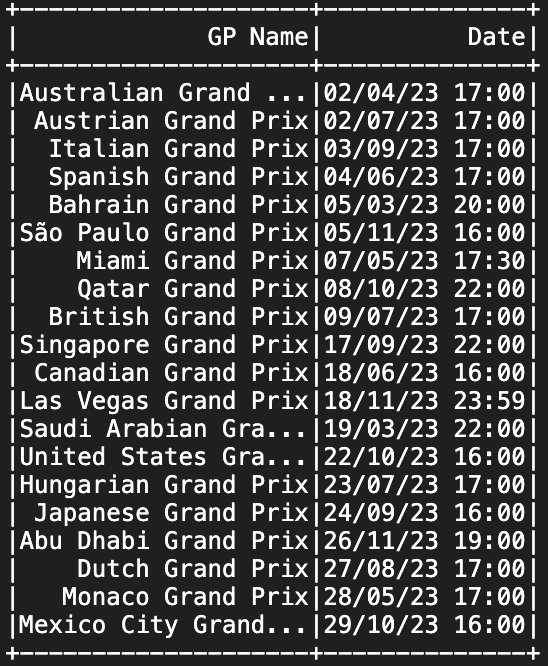
\includegraphics[width=0.5\textwidth]{ss-event-date.png}
    \caption{Event Dates Distribution GCP Querie Result}
\end{figure}

\begin{figure}[H]
    \centering
    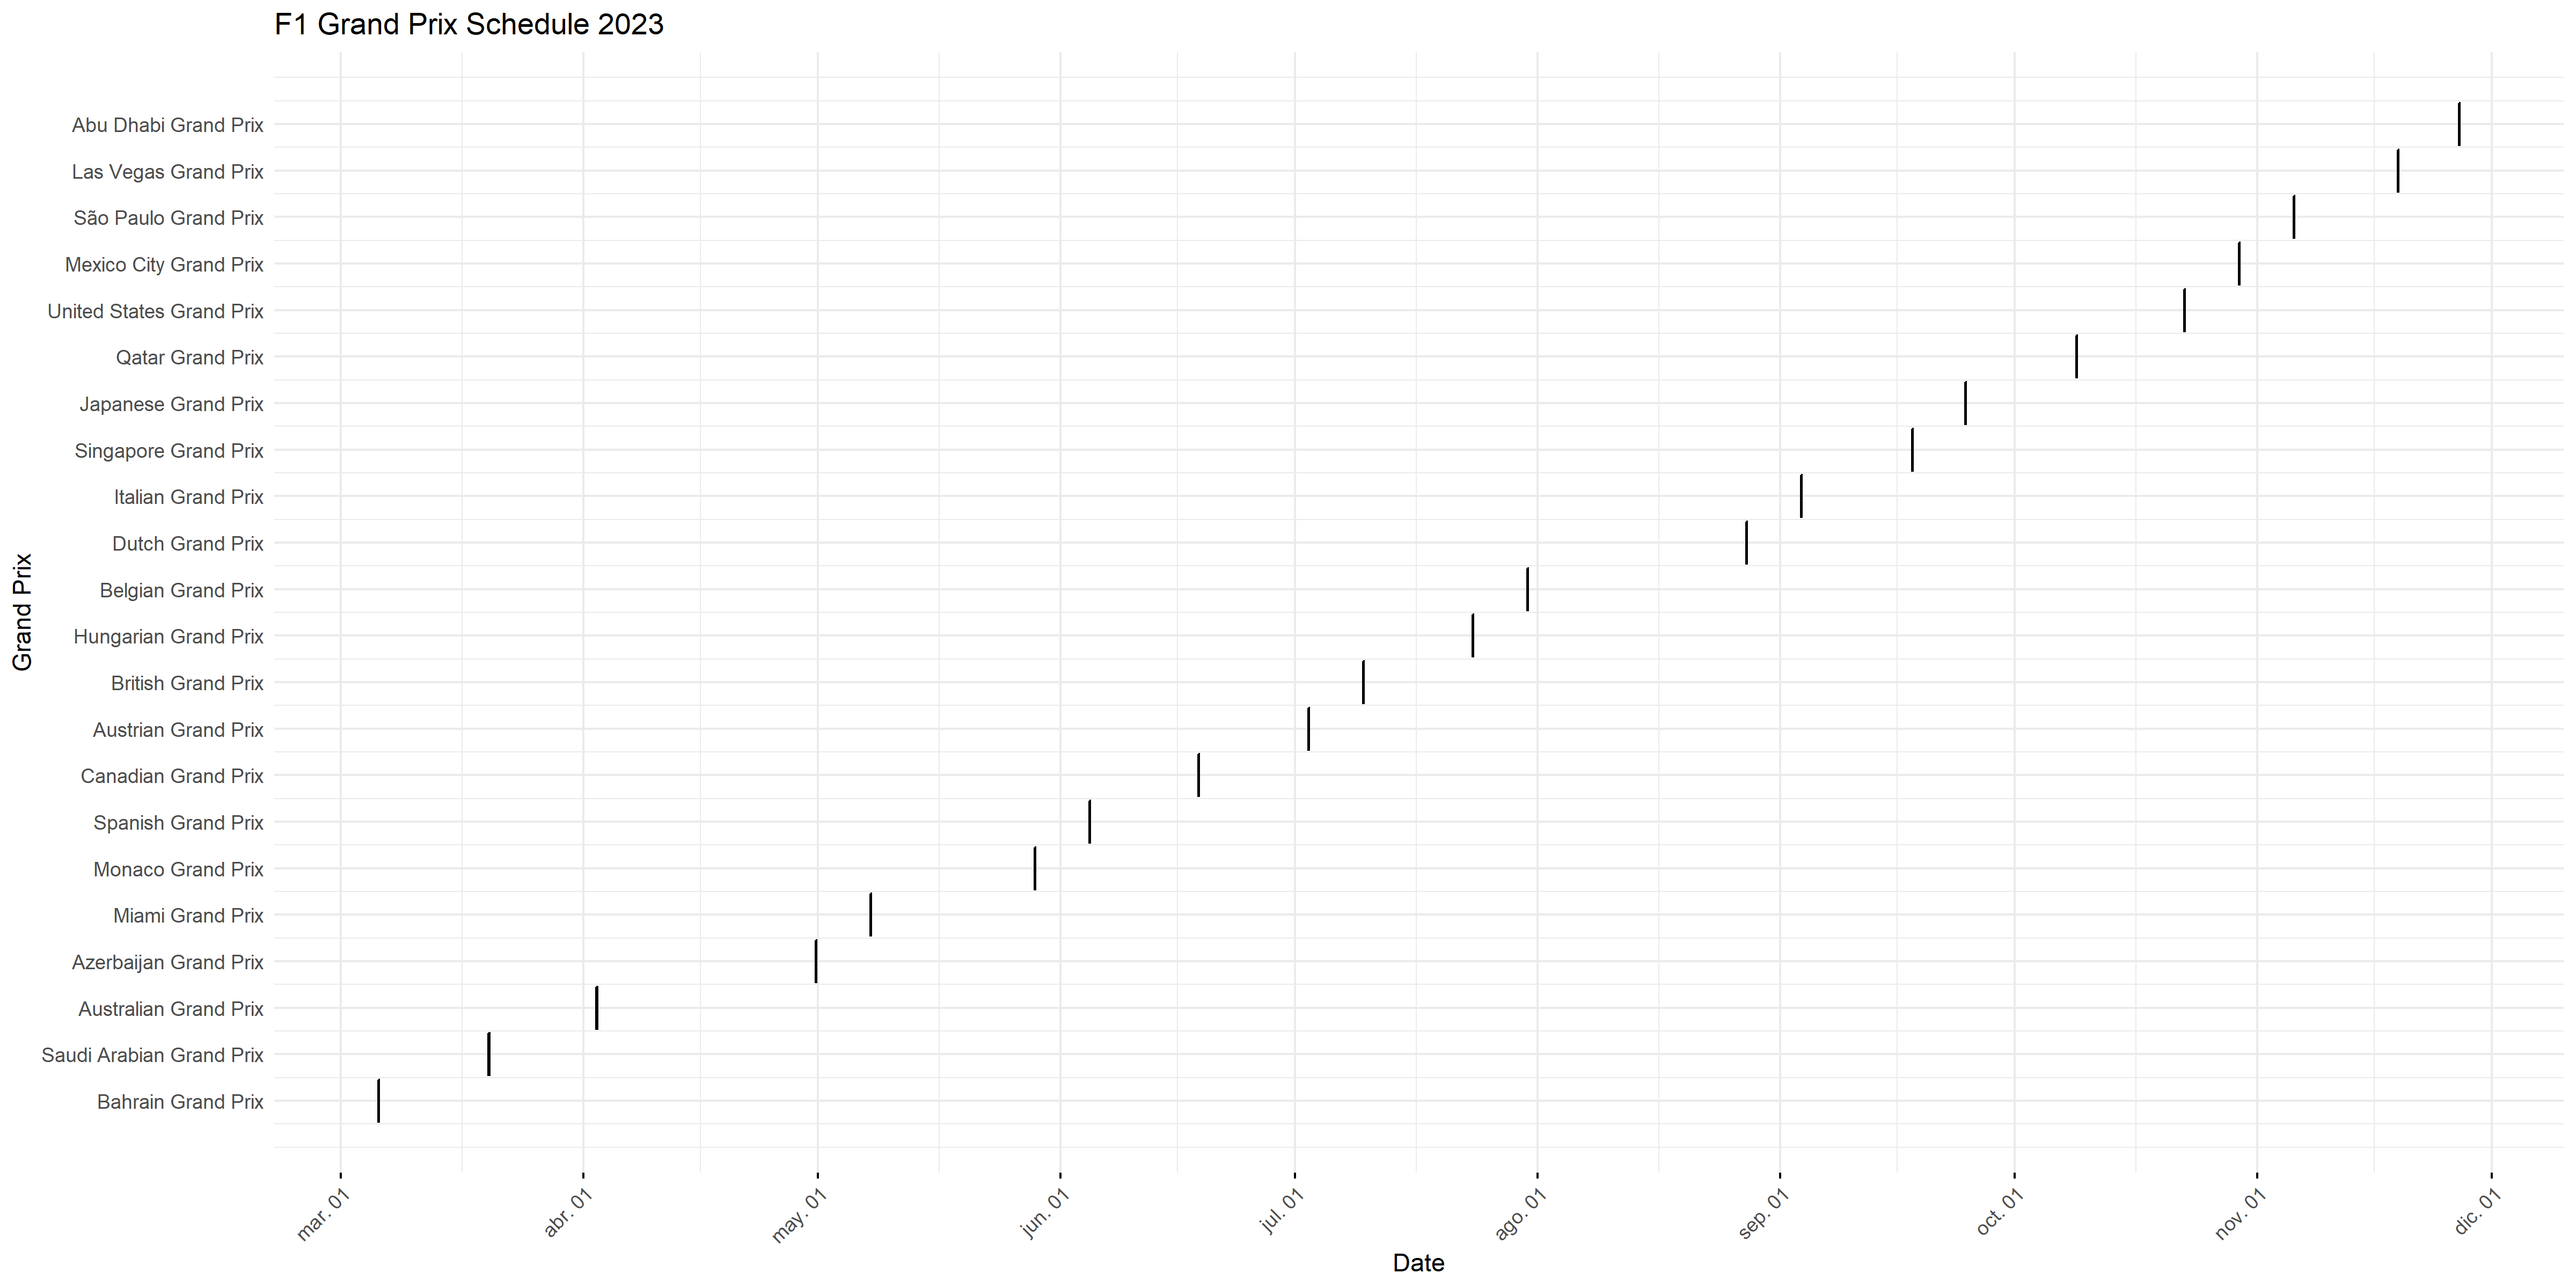
\includegraphics[width=\textwidth]{schedule_gantt.png}
    \caption{Gantt Chart of the F1 Grand Prix Schedule 2023}
\end{figure}

\paragraph{Interpretation:}
The Gantt chart illustrates the Formula 1 event schedule for the 2023 season. The timing of the races shows the workload and travel demands on the teams and drivers, highlighting periods with back-to-back races as well as breaks within the season. This information is crucial for teams to plan their logistics, training, and development activities efficiently.


\subsubsection{Total Laps by Tire Compound}
\paragraph{Description:}
This query categorizes the total number of laps completed on each tire compound, offering a clear depiction of tire utilization throughout the season. By examining the percentages of laps completed with each compound, teams can gain valuable insights into wear rates and preferences, which can significantly influence strategic decisions regarding tire management during races.

\begin{figure}[H]
    \centering
    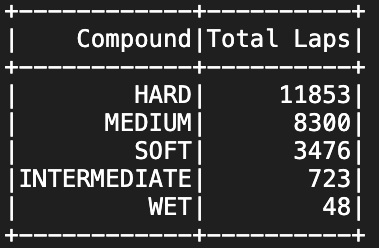
\includegraphics[width=0.4\textwidth]{ss-compound-laps.png}
    \caption{Total Laps per Compound GCP Querie Result}
\end{figure}

\begin{figure}[H]
    \centering
    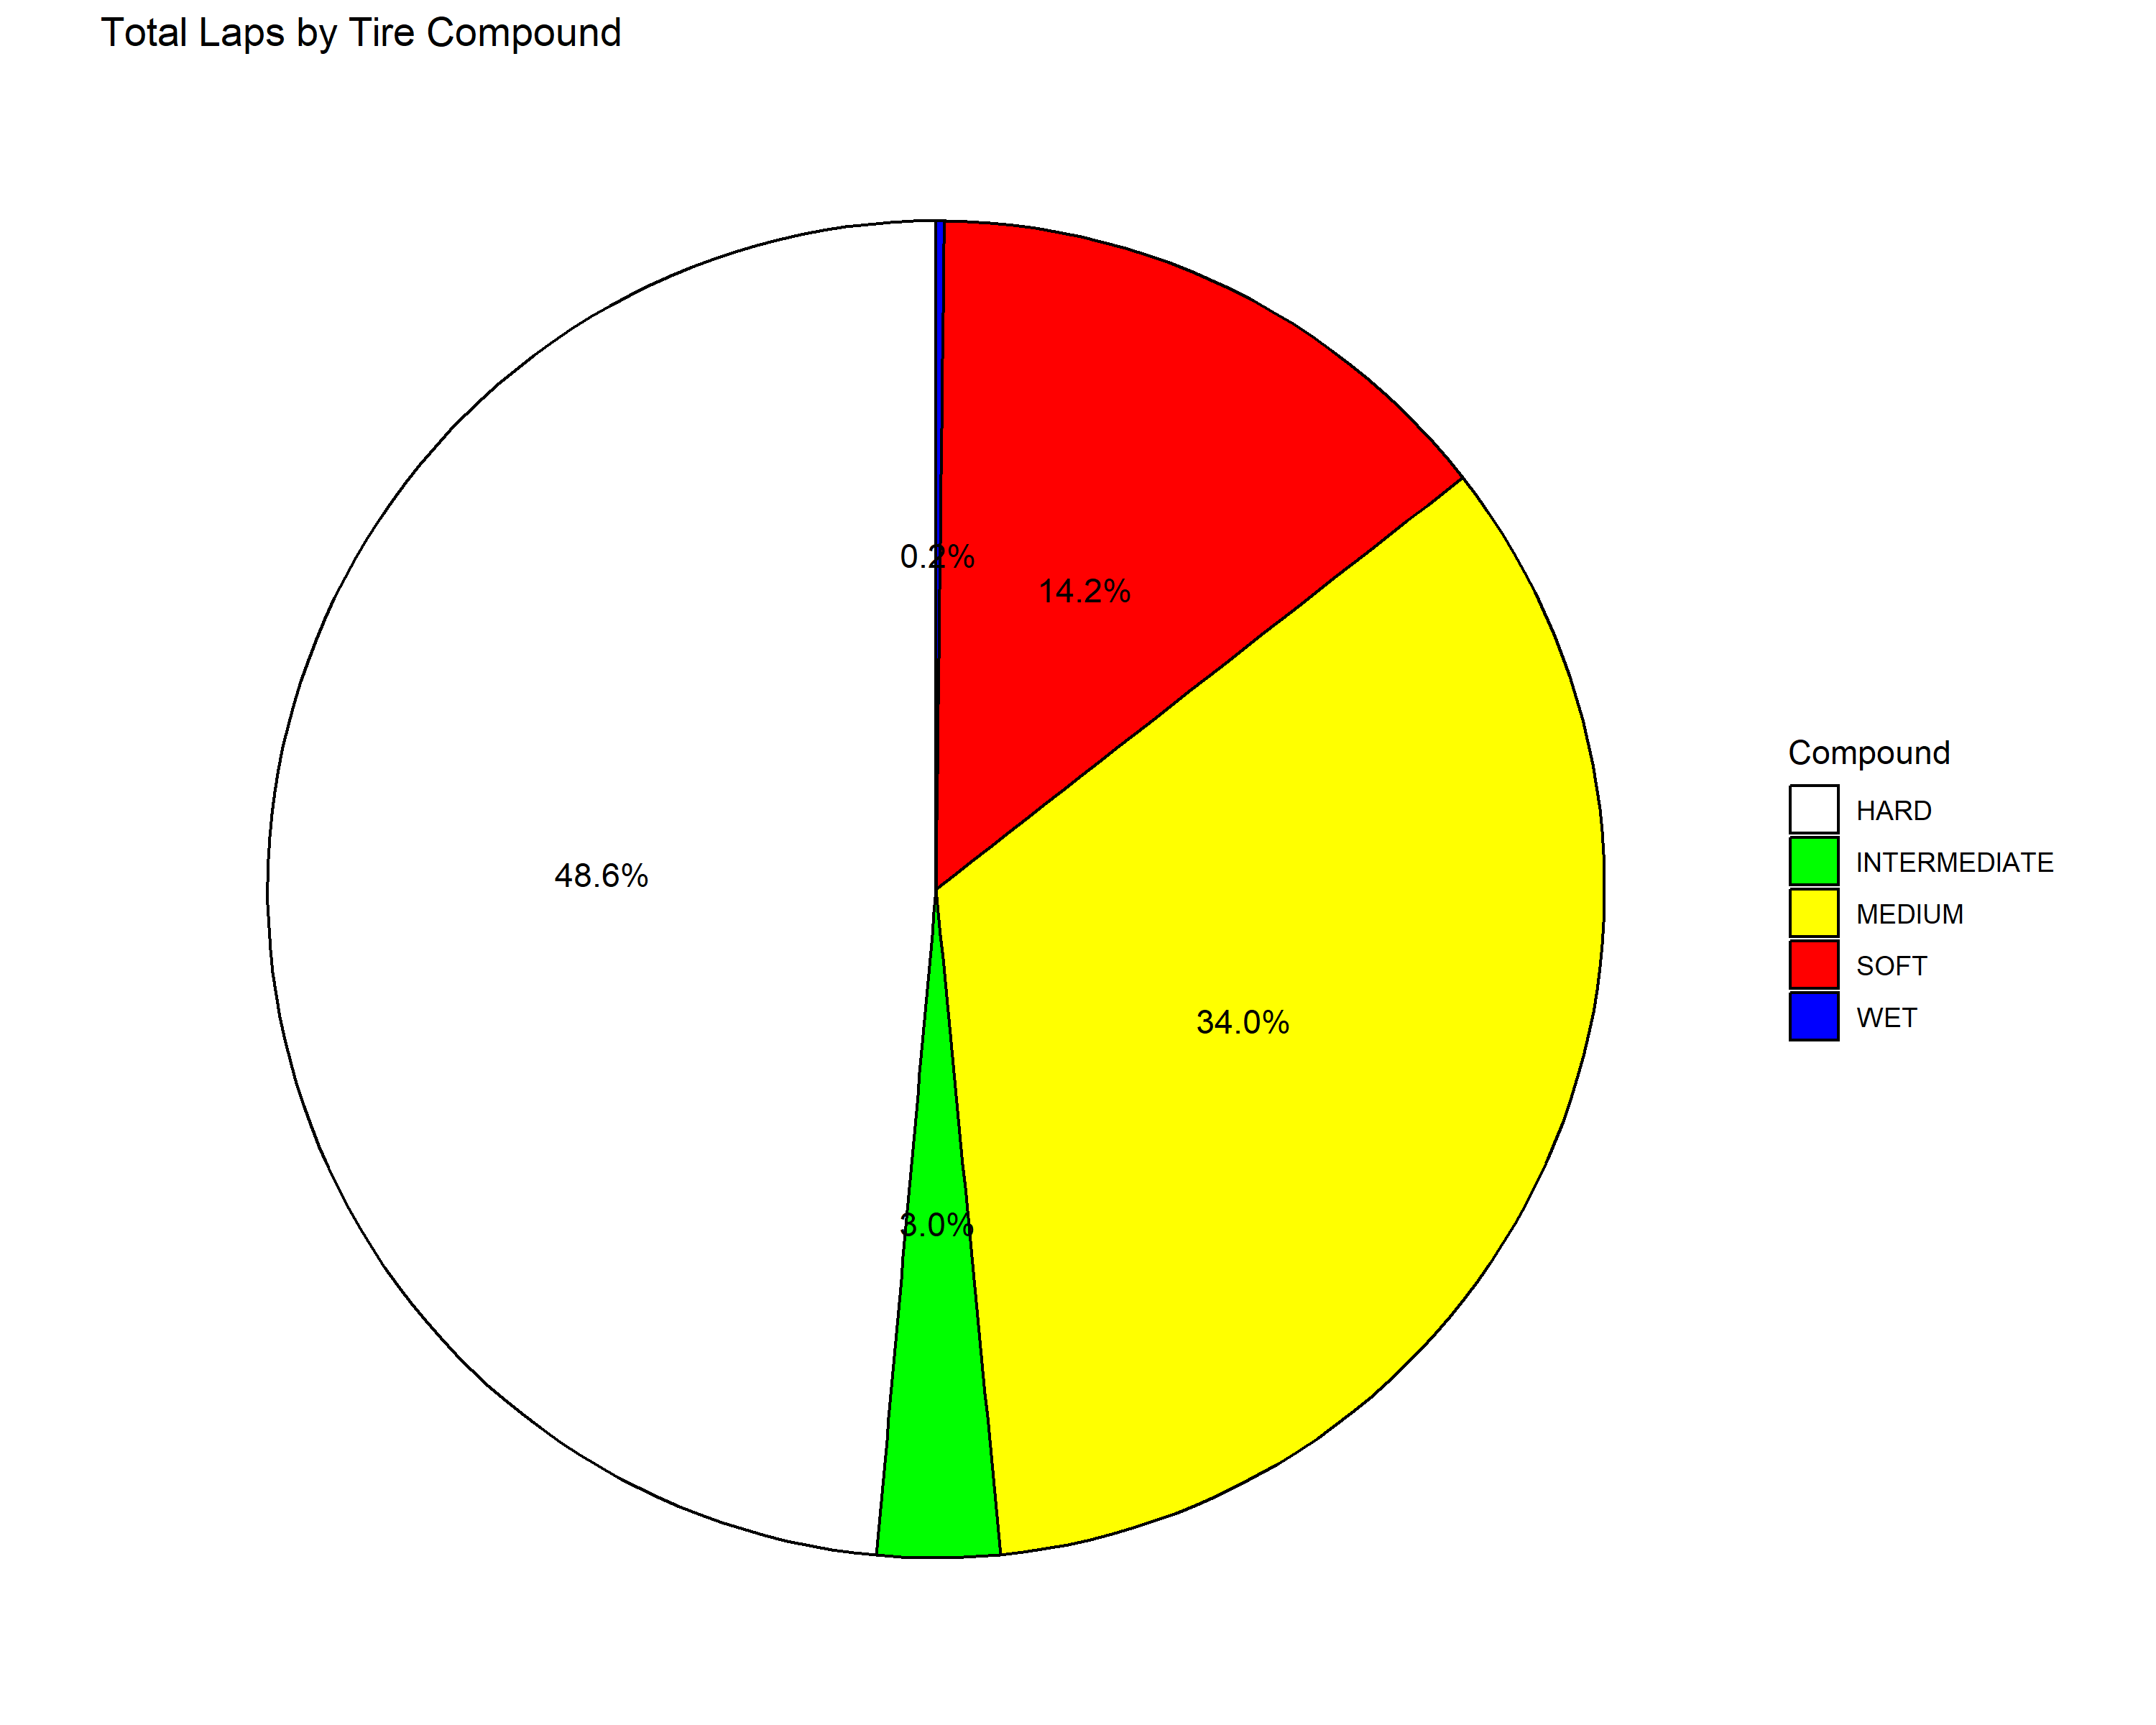
\includegraphics[width=0.8\textwidth]{total_laps_by_compound_pie_chart.png}
    \caption{Pie Chart of Total Laps by Tire Compound}
\end{figure}

\paragraph{Interpretation:}
The pie chart visually represents the proportion of total laps completed on different tire compounds throughout the season. The distribution can reflect not only a preference for certain compounds but also race conditions and regulations affecting tire choice. For example, a larger proportion of one compound could indicate its effectiveness or preference under specific race conditions.


\subsubsection{Number of Fastest Laps per Driver}
\paragraph{Description:}
This query calculates the total number of the fastest laps each driver achieved throughout the season, highlighting which drivers consistently performed at the top of their game during the critical moments of a race.

\begin{figure}[H]
    \centering
    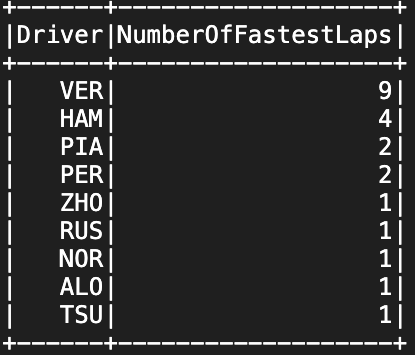
\includegraphics[width=0.4\textwidth]{ss-fast-laps.png}
    \caption{Fastest Laps per Driver GCP Query Result}
\end{figure}

\begin{figure}[H]
    \centering
    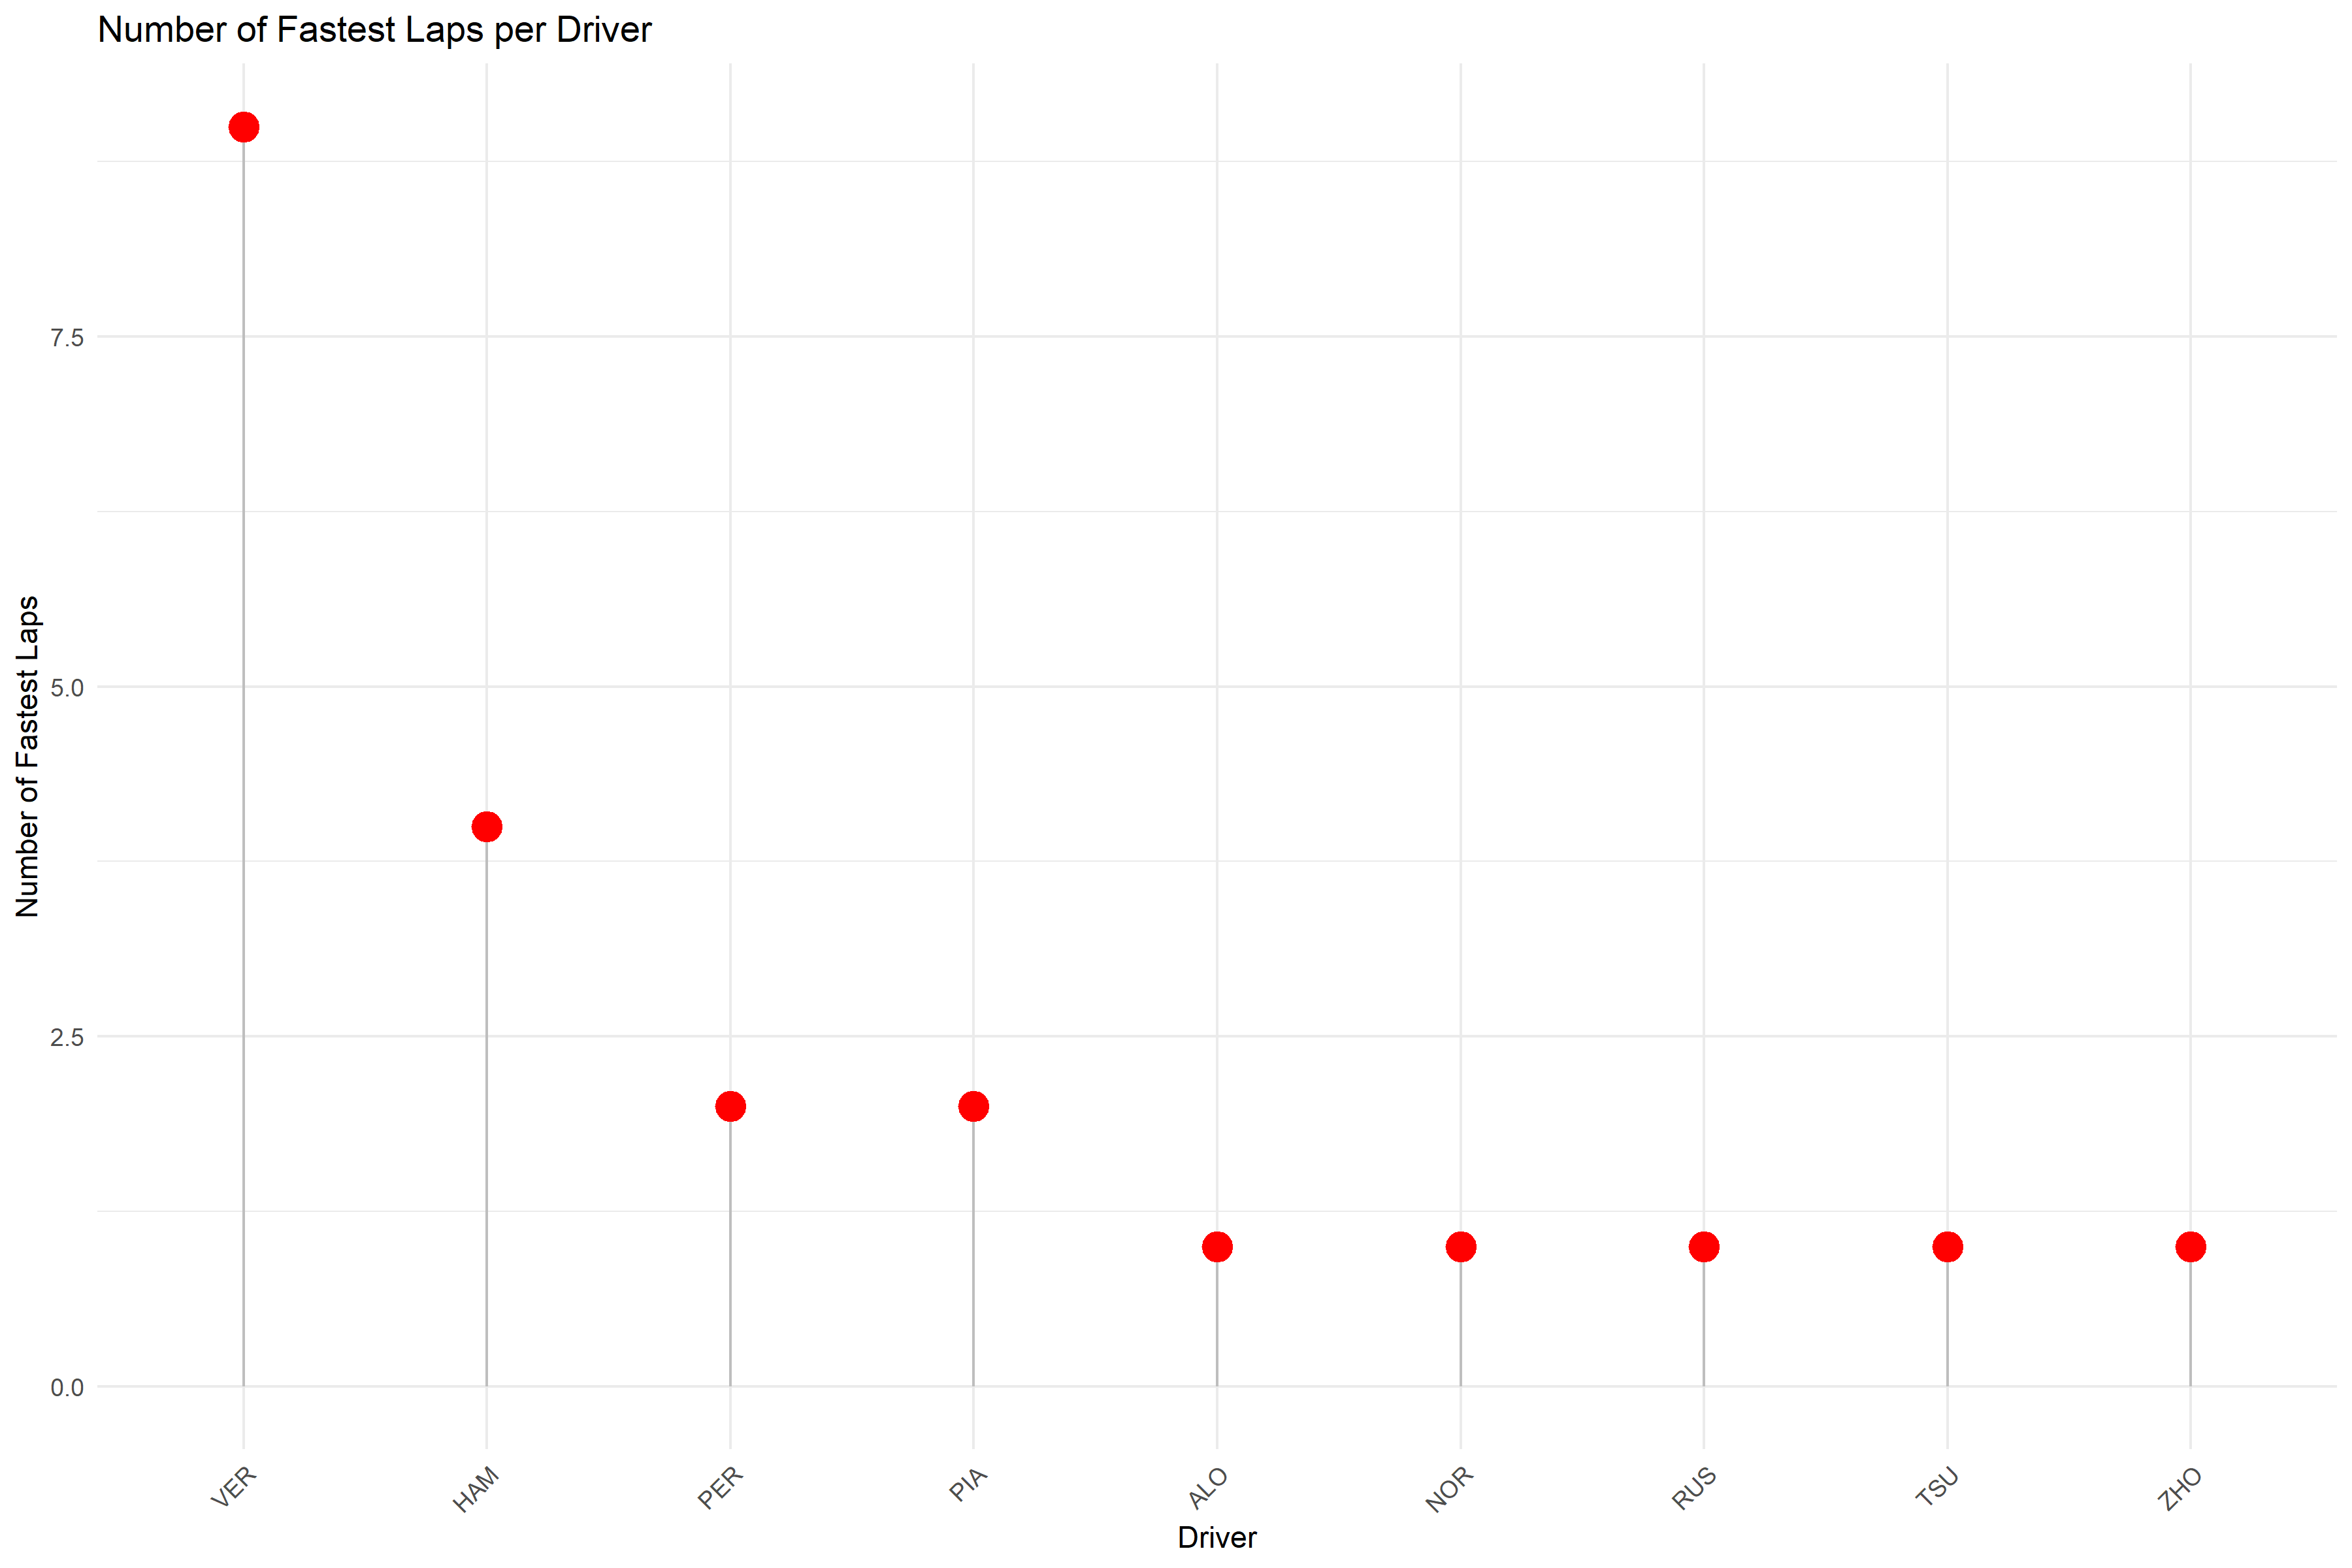
\includegraphics[width=\textwidth]{fastest_laps_lollipop.png}
    \caption{Lollipop Chart of the Number of Fastest Laps per Driver}
\end{figure}

\paragraph{Interpretation:}
The lollipop chart shows the number of fastest laps achieved by each driver, providing a clear visual of those who frequently led the pack. Drivers with a higher number of fastest laps may have a combination of skill, speed, and a well-performing car suited to the tracks, indicating their potential for success in races and qualifications.


\subsubsection{Driver Lap Completion Analysis}
\paragraph{Description:}
This query analyzes each driver's completed versus incomplete laps, expressed both in absolute terms and as percentages. It highlights drivers' reliability and consistency during races. For this analysis, we applied a rigorous data validation approach similar to one previously mentioned. This step was crucial to confirm the precision of our dataset, particularly in distinguishing between non-existent (null) and explicitly recorded empty lap times. A thorough explanation of this validation technique will be provided in the upcoming segments.

\begin{figure}[H]
    \centering
    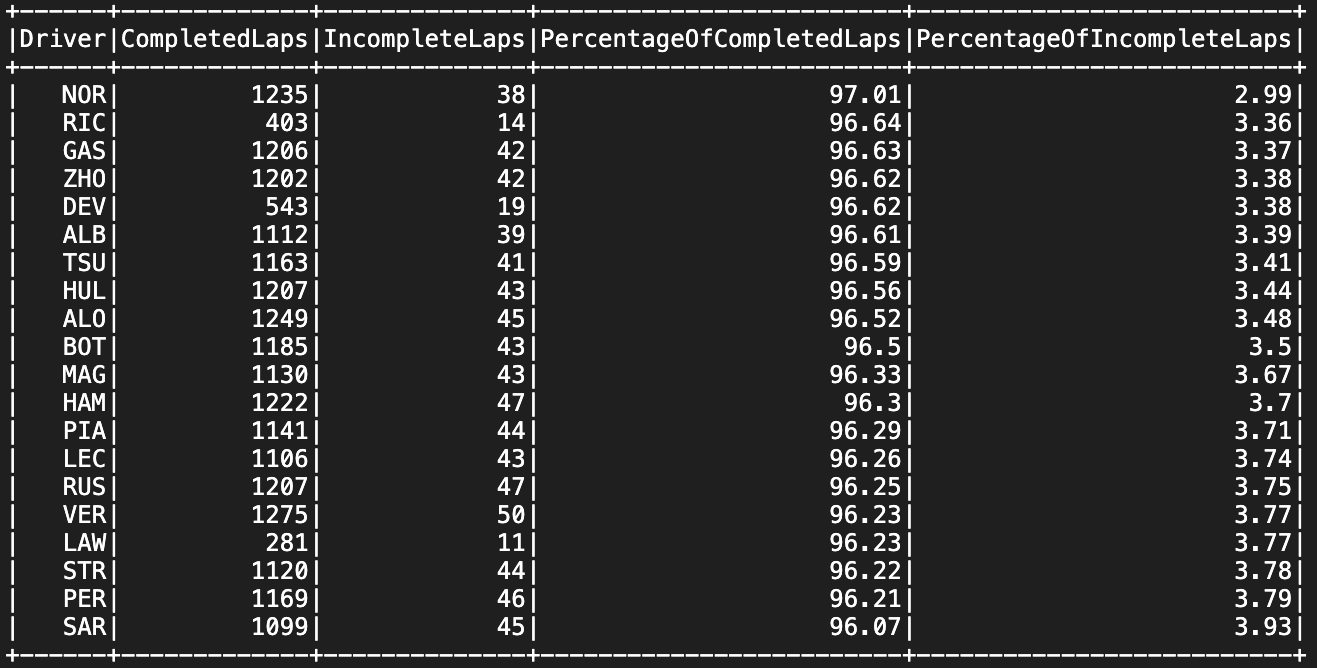
\includegraphics[width=\textwidth]{complete-percentage.png}
    \caption{Driver Lap Completion Rate GCP Querie Result}
\end{figure}

\begin{figure}[H]
    \centering
    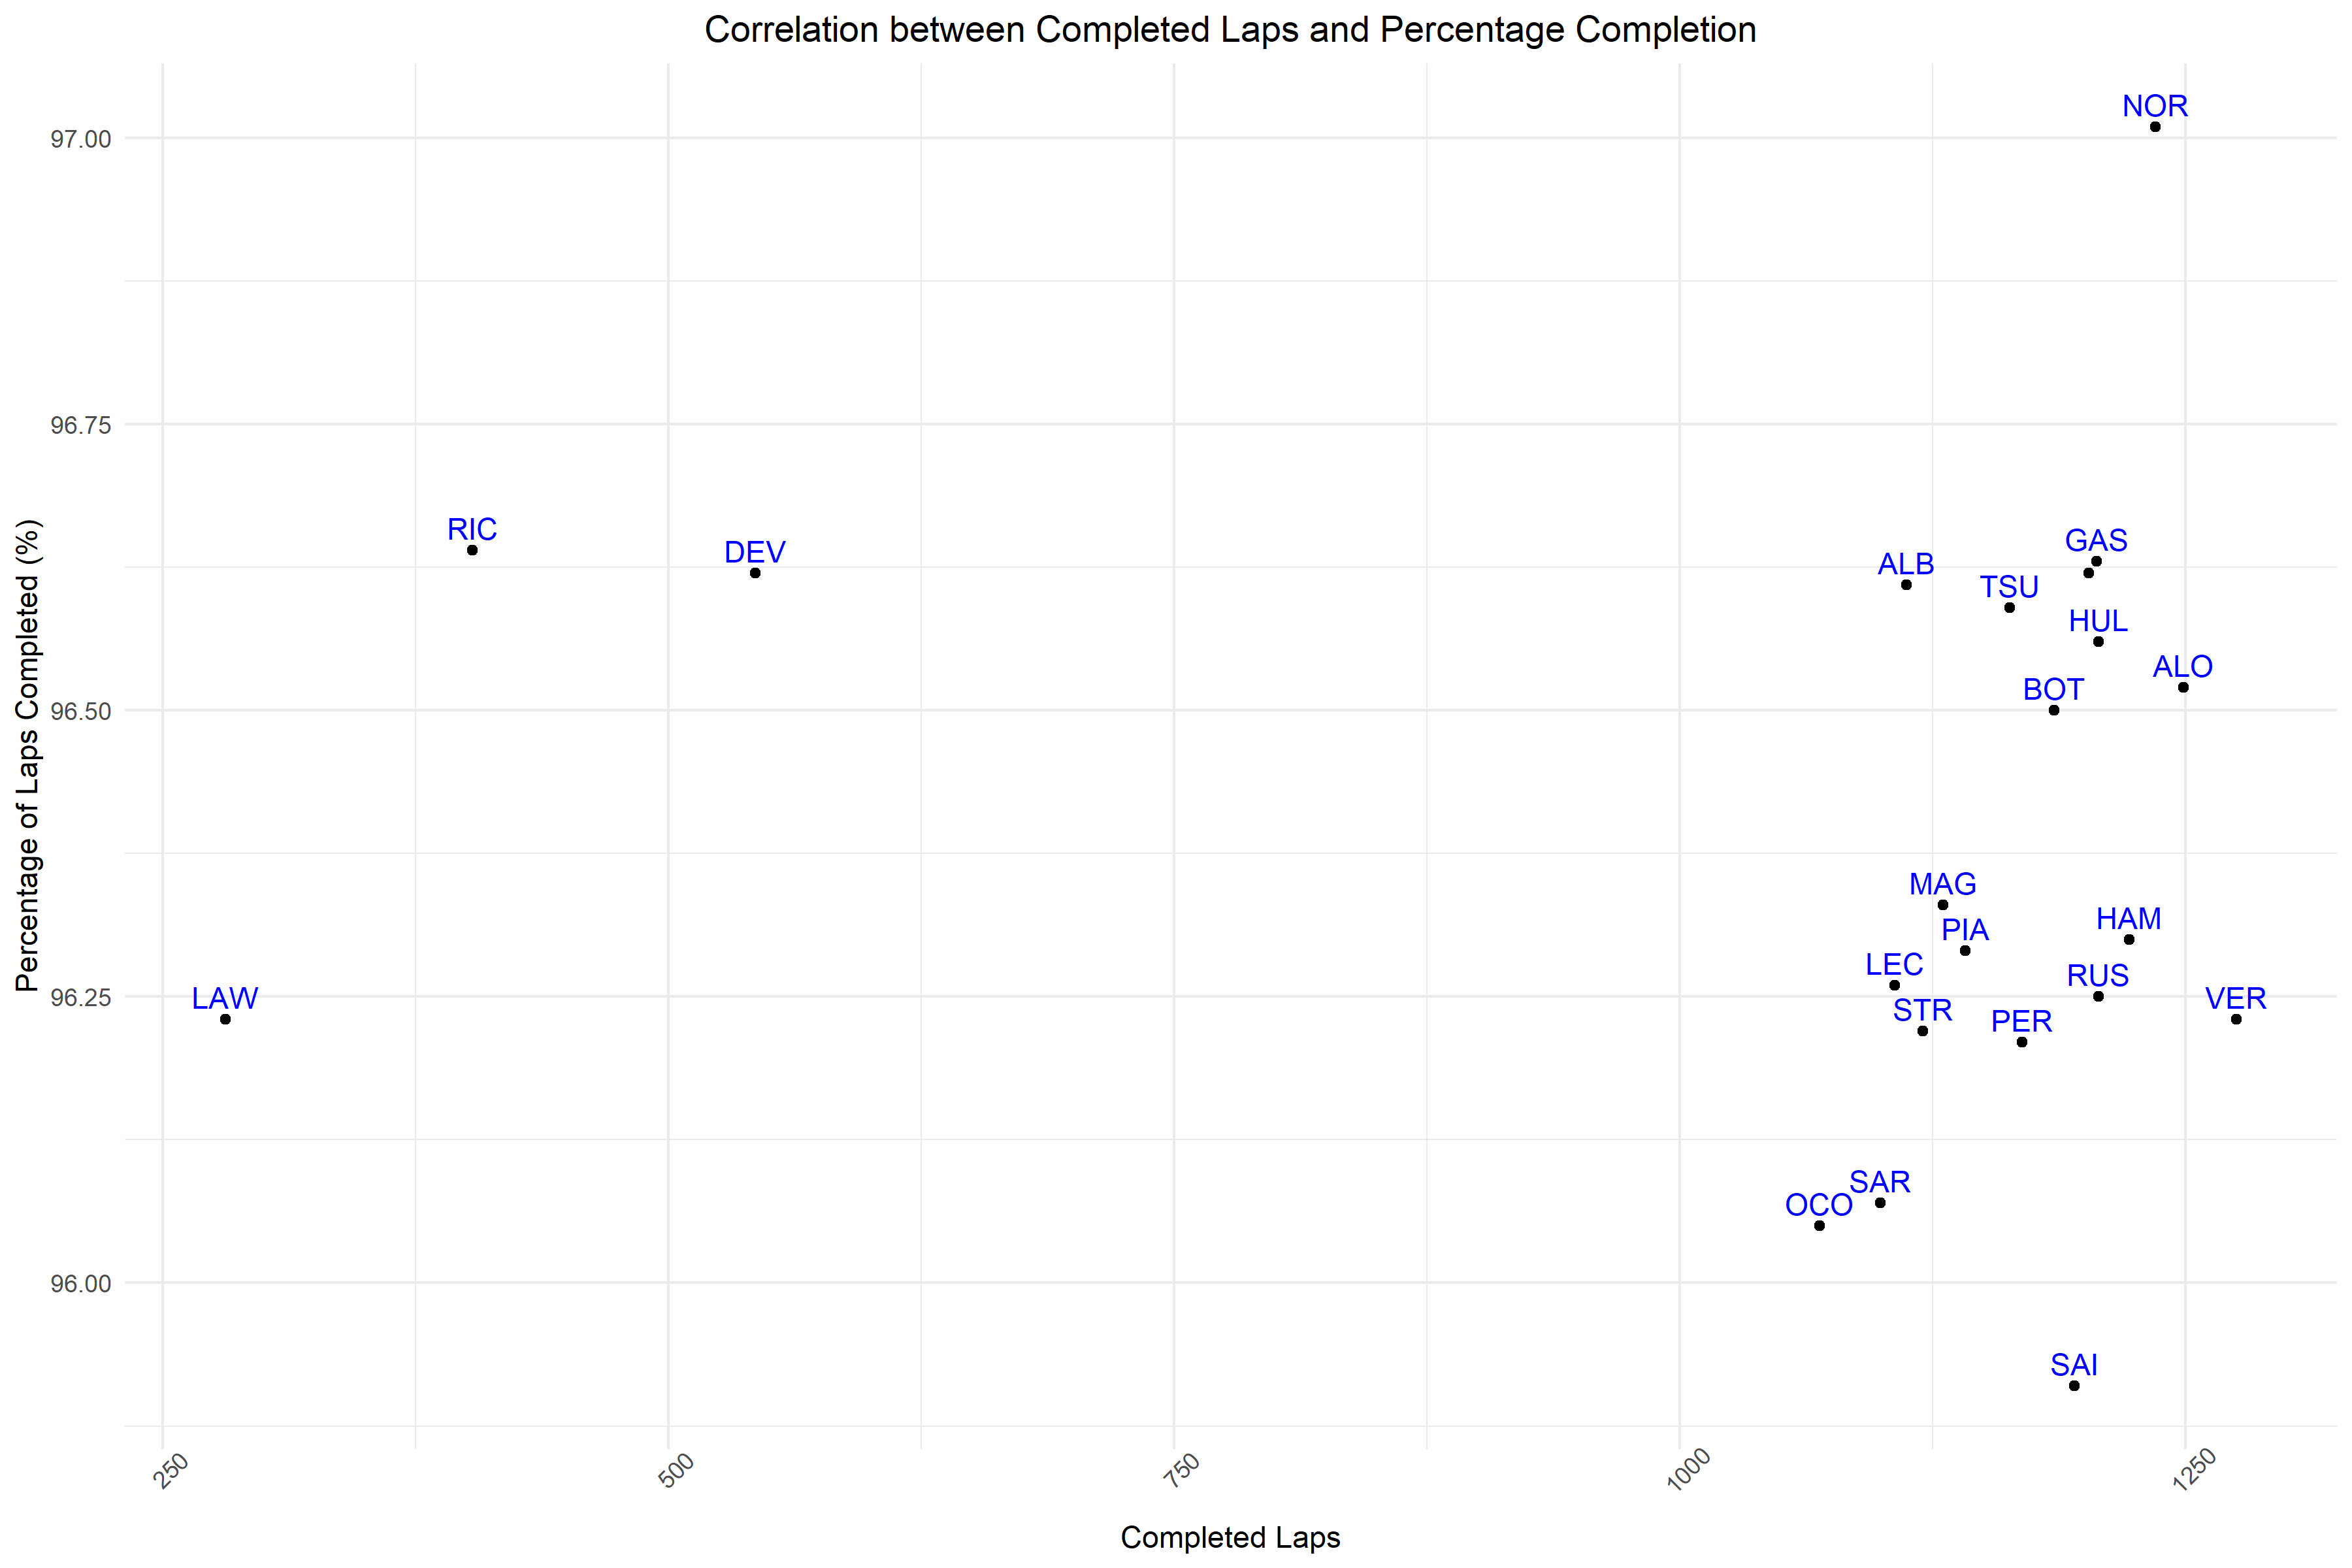
\includegraphics[width=\textwidth]{driver_lap_completion_scatter_plot.png}
    \caption{Scatter Plot of Driver Lap Completion Rates}
\end{figure}

\paragraph{Interpretation:}
The scatter plot showcases the completion rate of laps for each driver across the season, providing insights into which drivers are more likely to finish laps, and hence, potentially races. This measure of consistency is essential for teams when evaluating driver performance and endurance over the season.

\subsubsection{Telemetry Analysis by Driver and Event}
\paragraph{Description:}
This query delves into telemetry data to extract average throttle usage, braking frequency, speed statistics, RPM levels, and DRS activation percentages for each driver across events. Such analysis paints a comprehensive picture of driving styles and car performance under different race conditions.

\begin{figure}[H]
    \centering
    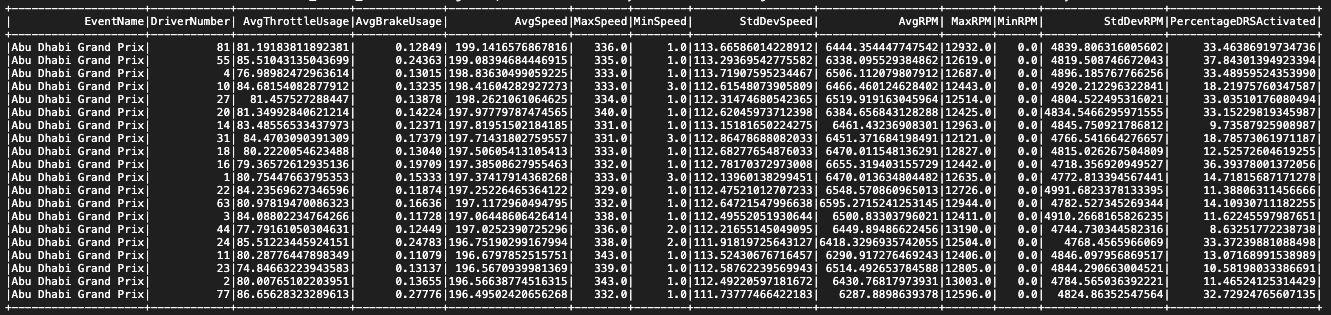
\includegraphics[width=\textwidth]{telemetry.png}
    \caption{Event Telemetry GCP Querie Result}
\end{figure}

\begin{figure}[H]
    \centering
    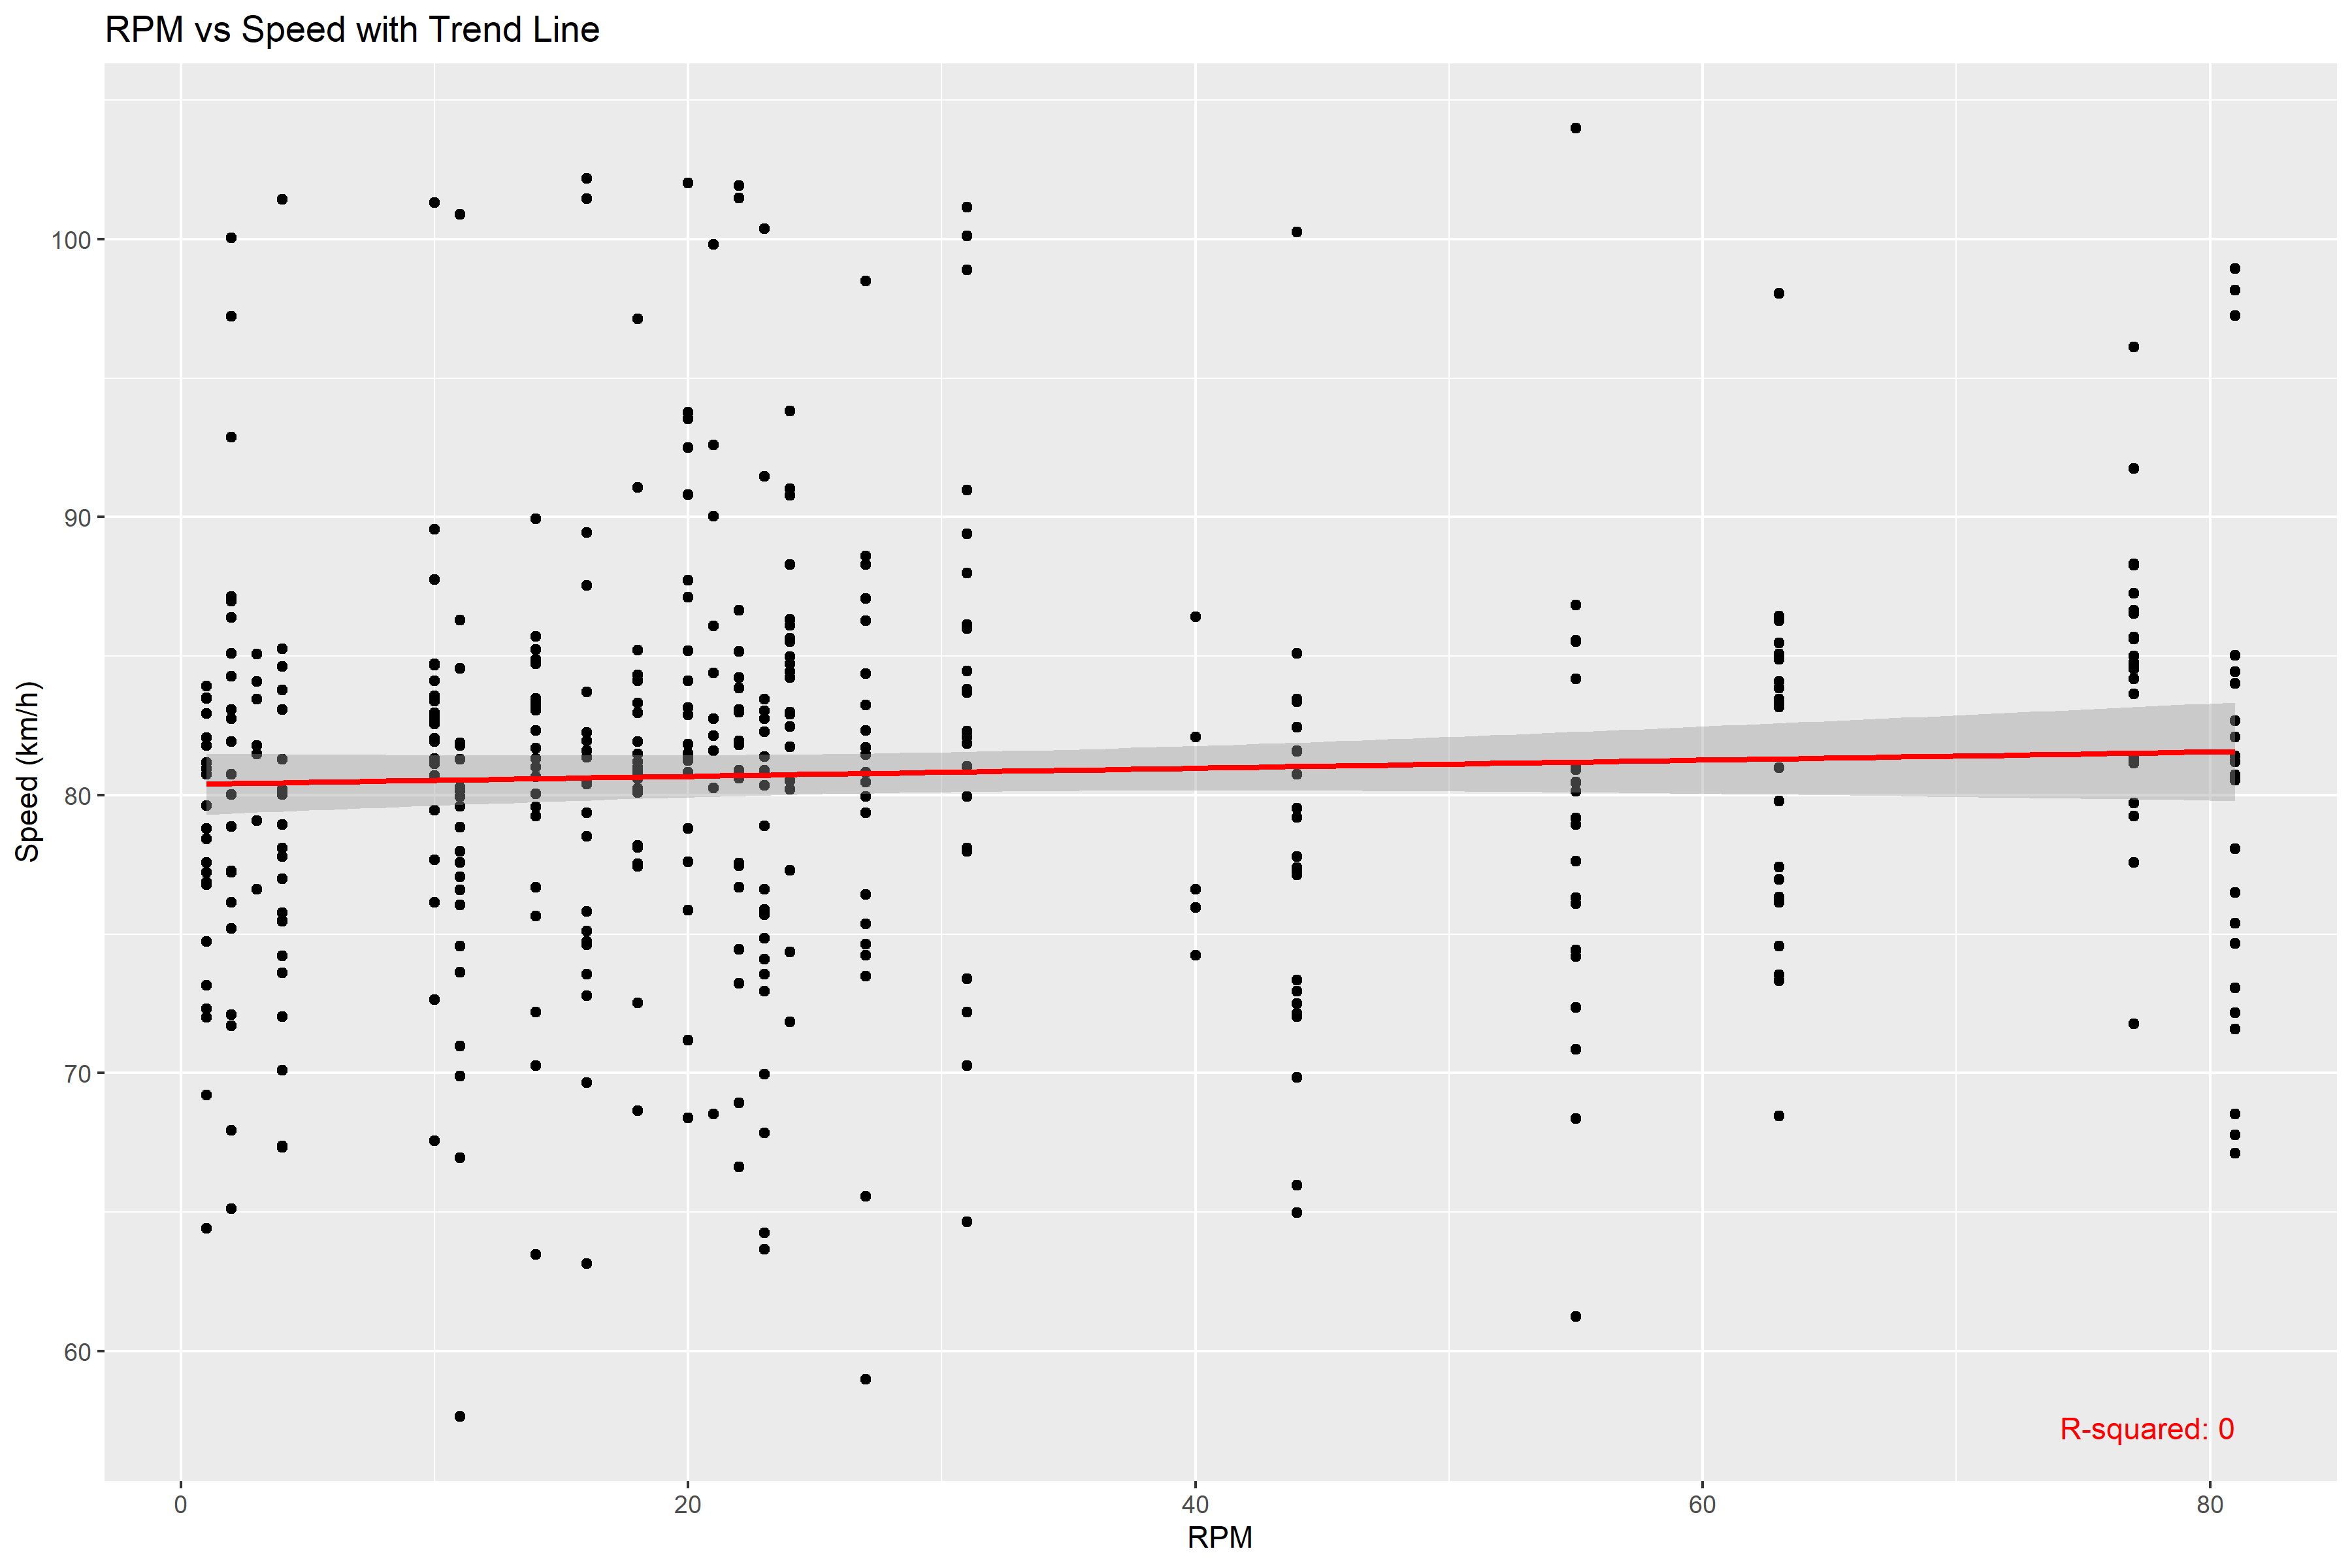
\includegraphics[width=\textwidth]{avg_speed_vs_rpm.png}
    \caption{Scatter Plot with Trend Line: RPM vs Speed Analysis}
\end{figure}

\paragraph{Interpretation:}
The scatter plot with the overlaying trend line represents the relationship between RPM (revolutions per minute) and the speed of the vehicles. Despite the variability, the trend line suggests a weak positive correlation; however, with an R-squared value of 0, this indicates no predictive power. This could suggest that factors other than RPM may have a more significant influence on speed, or it could reflect a variety of driving styles and strategies employed by the drivers. Additionally, the spread of data points might indicate differing car performances or the impact of track conditions.



\subsubsection{Correlation between Lap Times by Tire Compound and Weather Conditions}
\paragraph{Description:}
This analysis investigates the interaction between tire compound choices and weather conditions, looking at average lap times. Through the use of window functions in Spark SQL, we've been able to categorize weather conditions and directly correlate them with performance metrics such as average lap times for different tire compounds.

\begin{figure}[H]
    \centering
    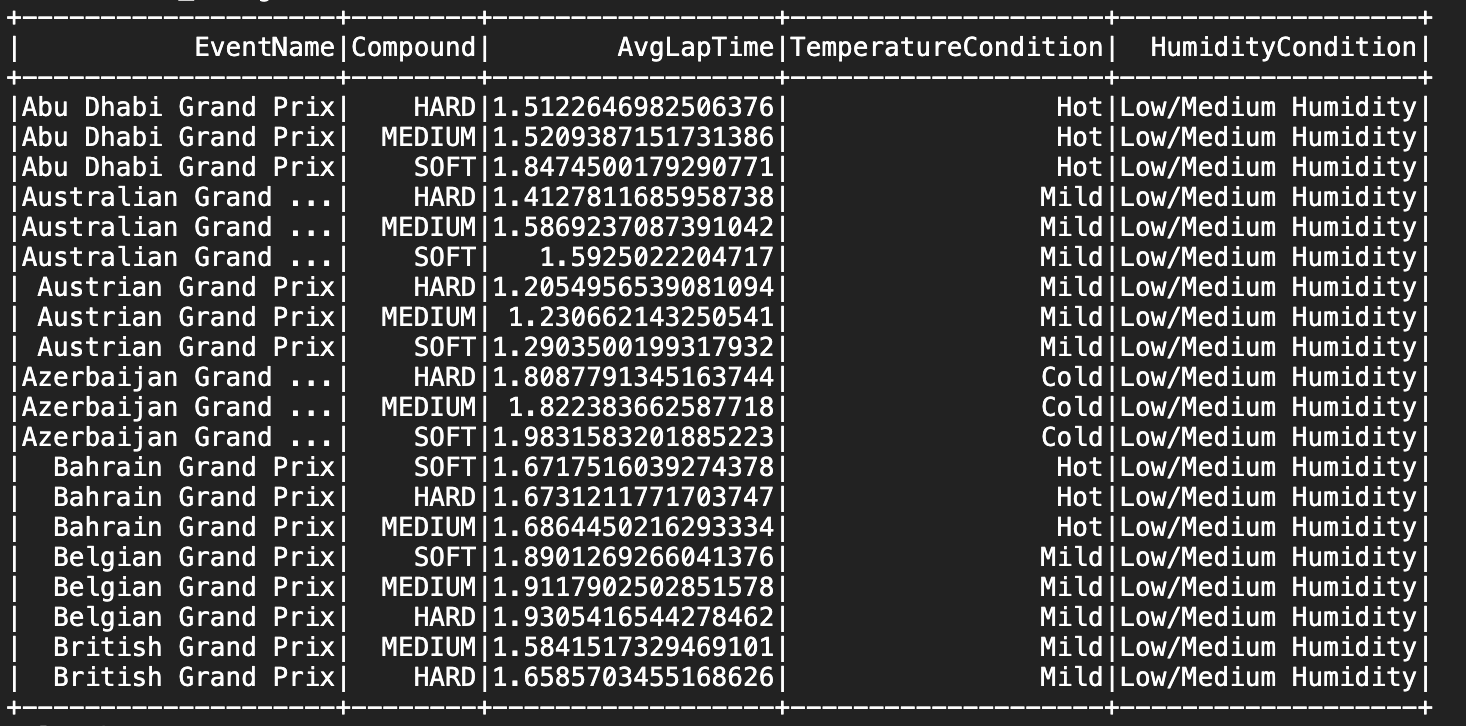
\includegraphics[width=\textwidth]{weather.png}
    \caption{Weather Insights per Event GCP Querie Result}
\end{figure}

\begin{figure}[H]
    \centering
    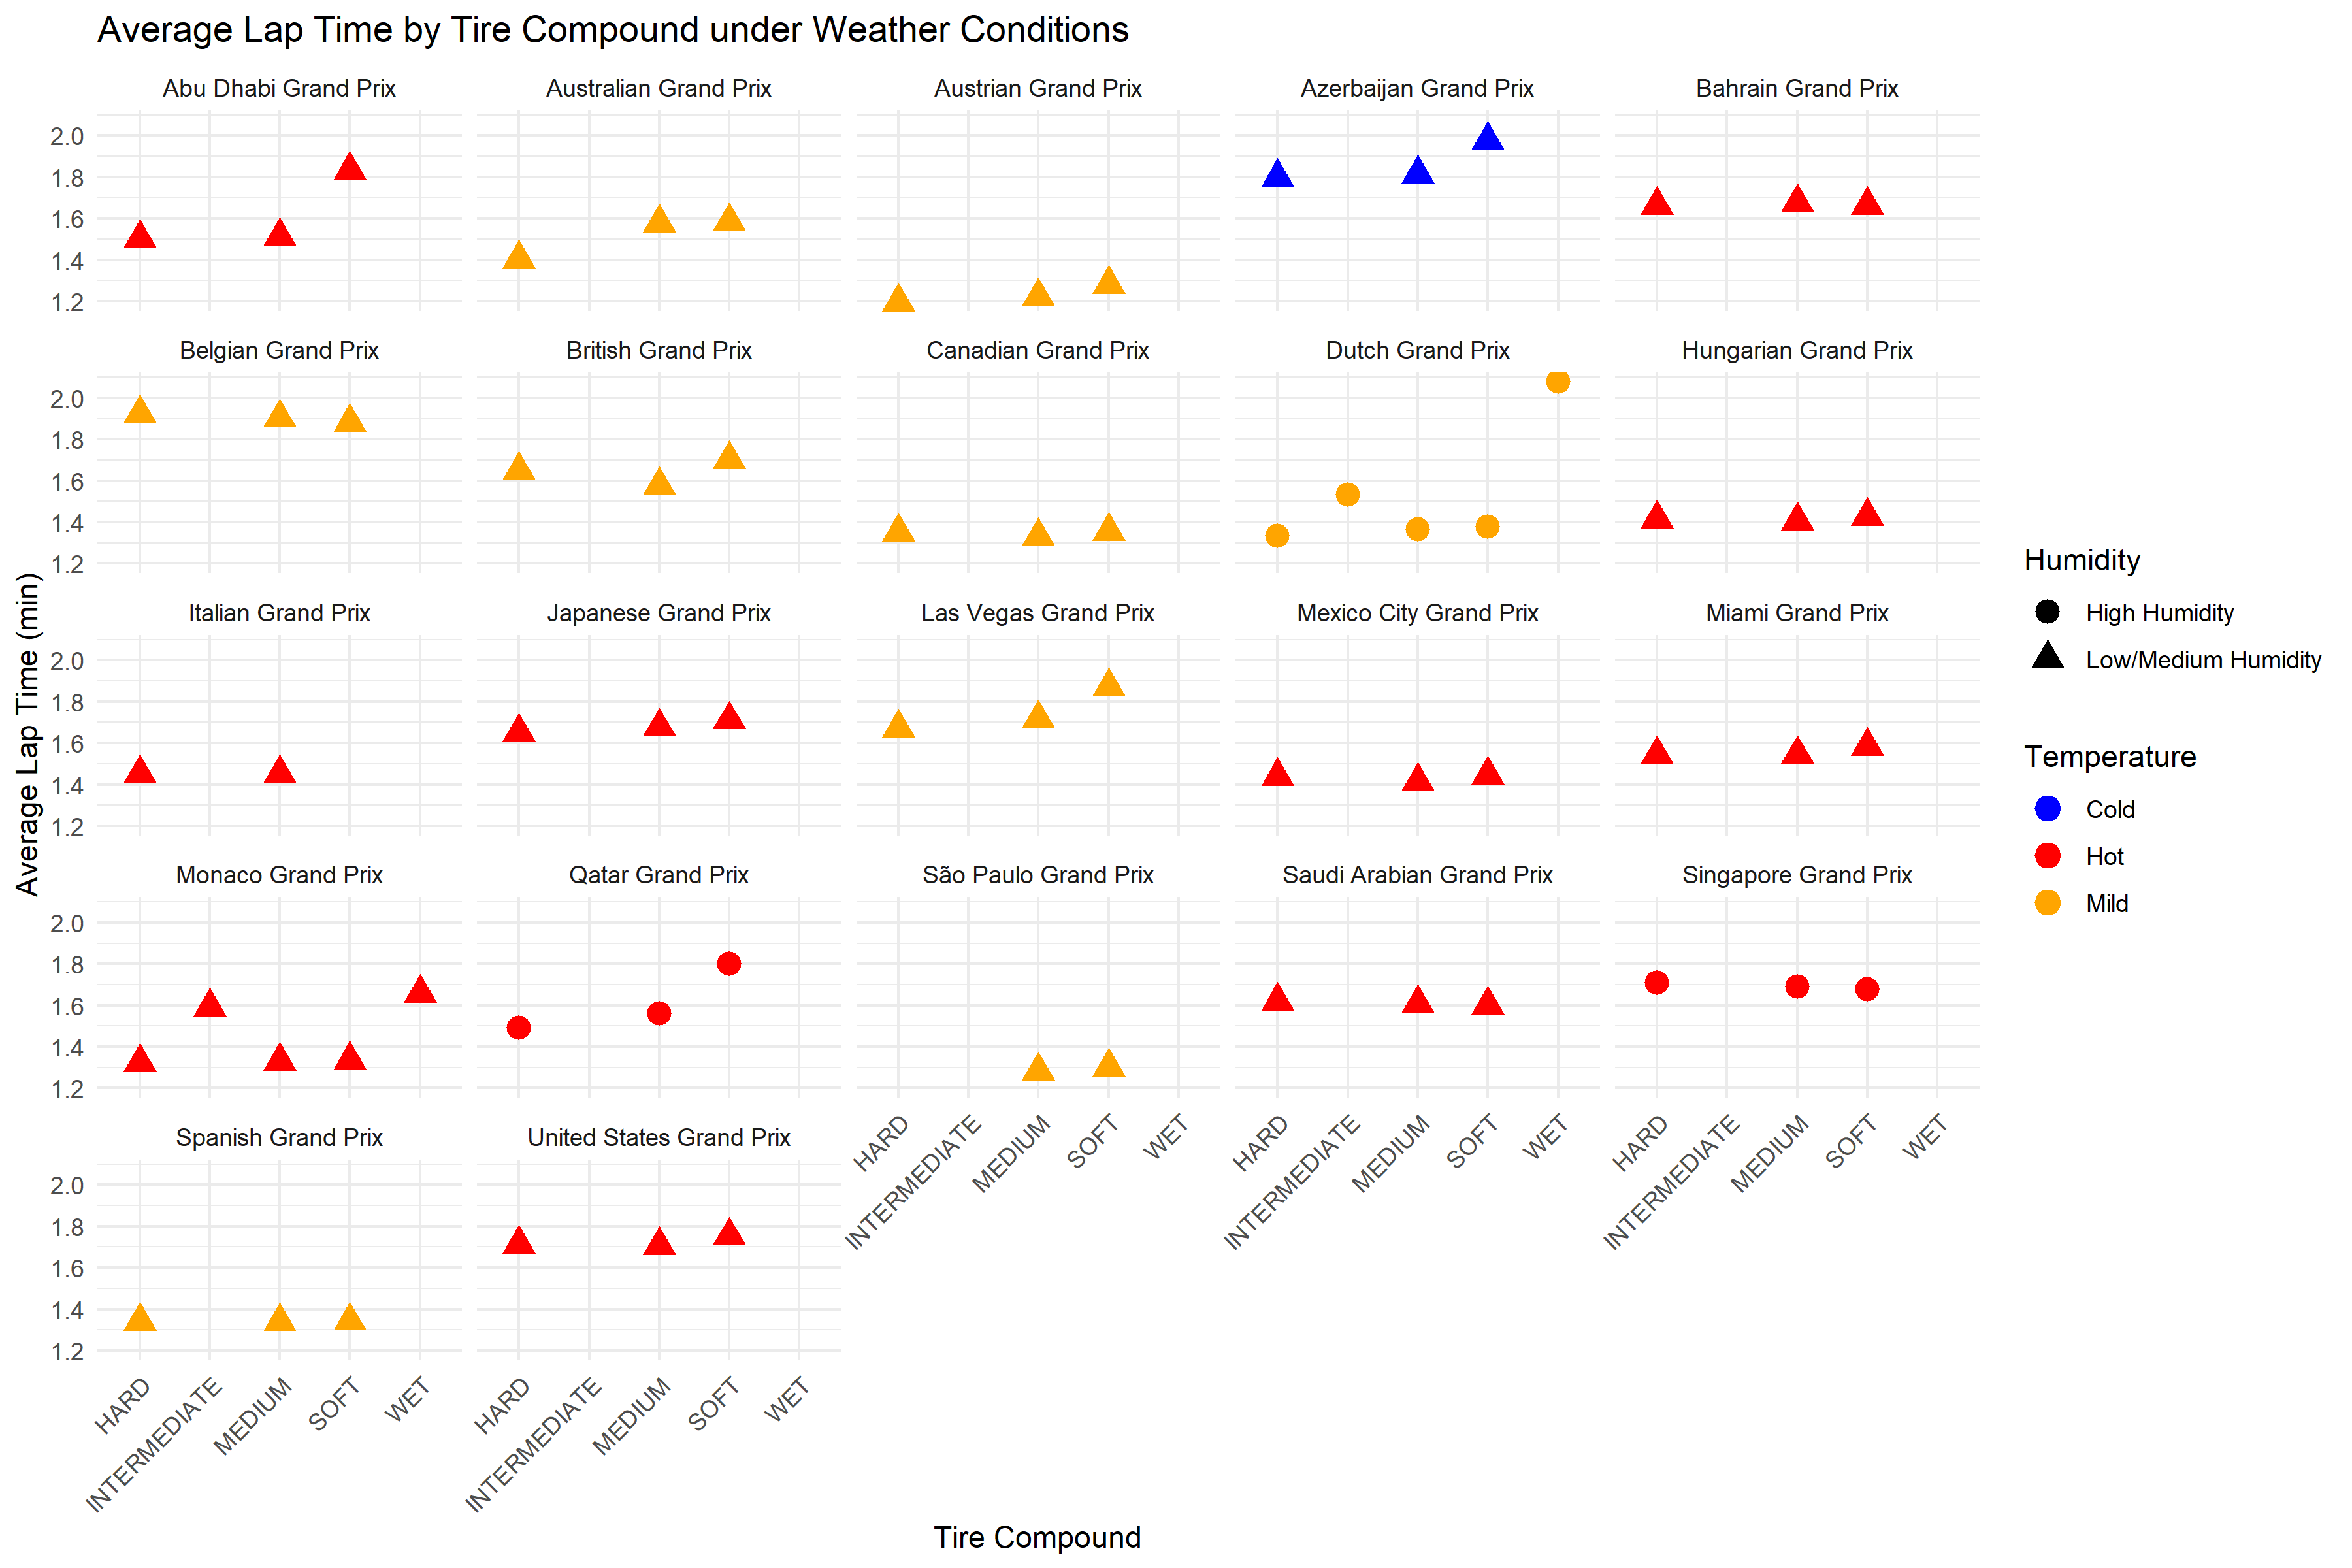
\includegraphics[width=\textwidth]{performance_weather_conditions_interaction_plot.png}
    \caption{Interaction Plot of Performance vs. Weather Conditions}
\end{figure}

\paragraph{Interpretation:}
The interaction plot demonstrates how tire compounds perform under various temperature and humidity conditions during different Grand Prix events. Circular markers for 'High Humidity' and triangular for varying temperature conditions give a visual representation of their impact on lap times. This kind of analysis is essential for teams to adapt their strategies, such as tire choices and car setups, to the predicted weather on a race day.


\subsubsection{Dot Chart Overview by Driver}
\paragraph{Description:}
This analysis offers a visualization of average lap times juxtaposed with the completion rate and the most used tire compounds for each driver. It serves as a way to observe correlations between performance and tire choices.

\begin{figure}[H]
    \centering
    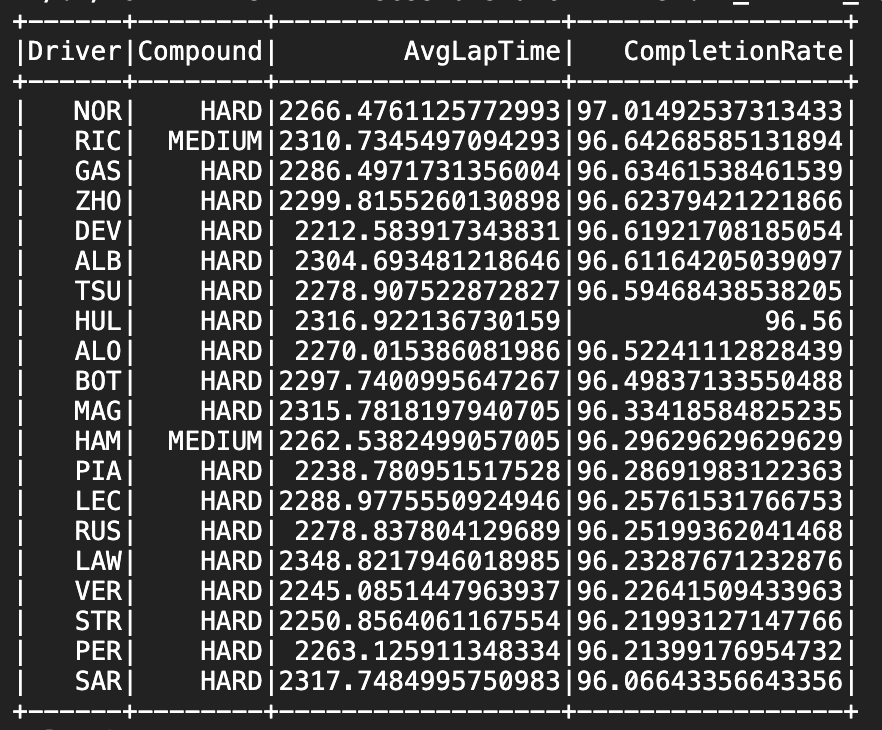
\includegraphics[width=\textwidth]{ovw.png}
    \caption{Driver Overview GCP Querie Result }
\end{figure}

\begin{figure}[H]
    \centering
    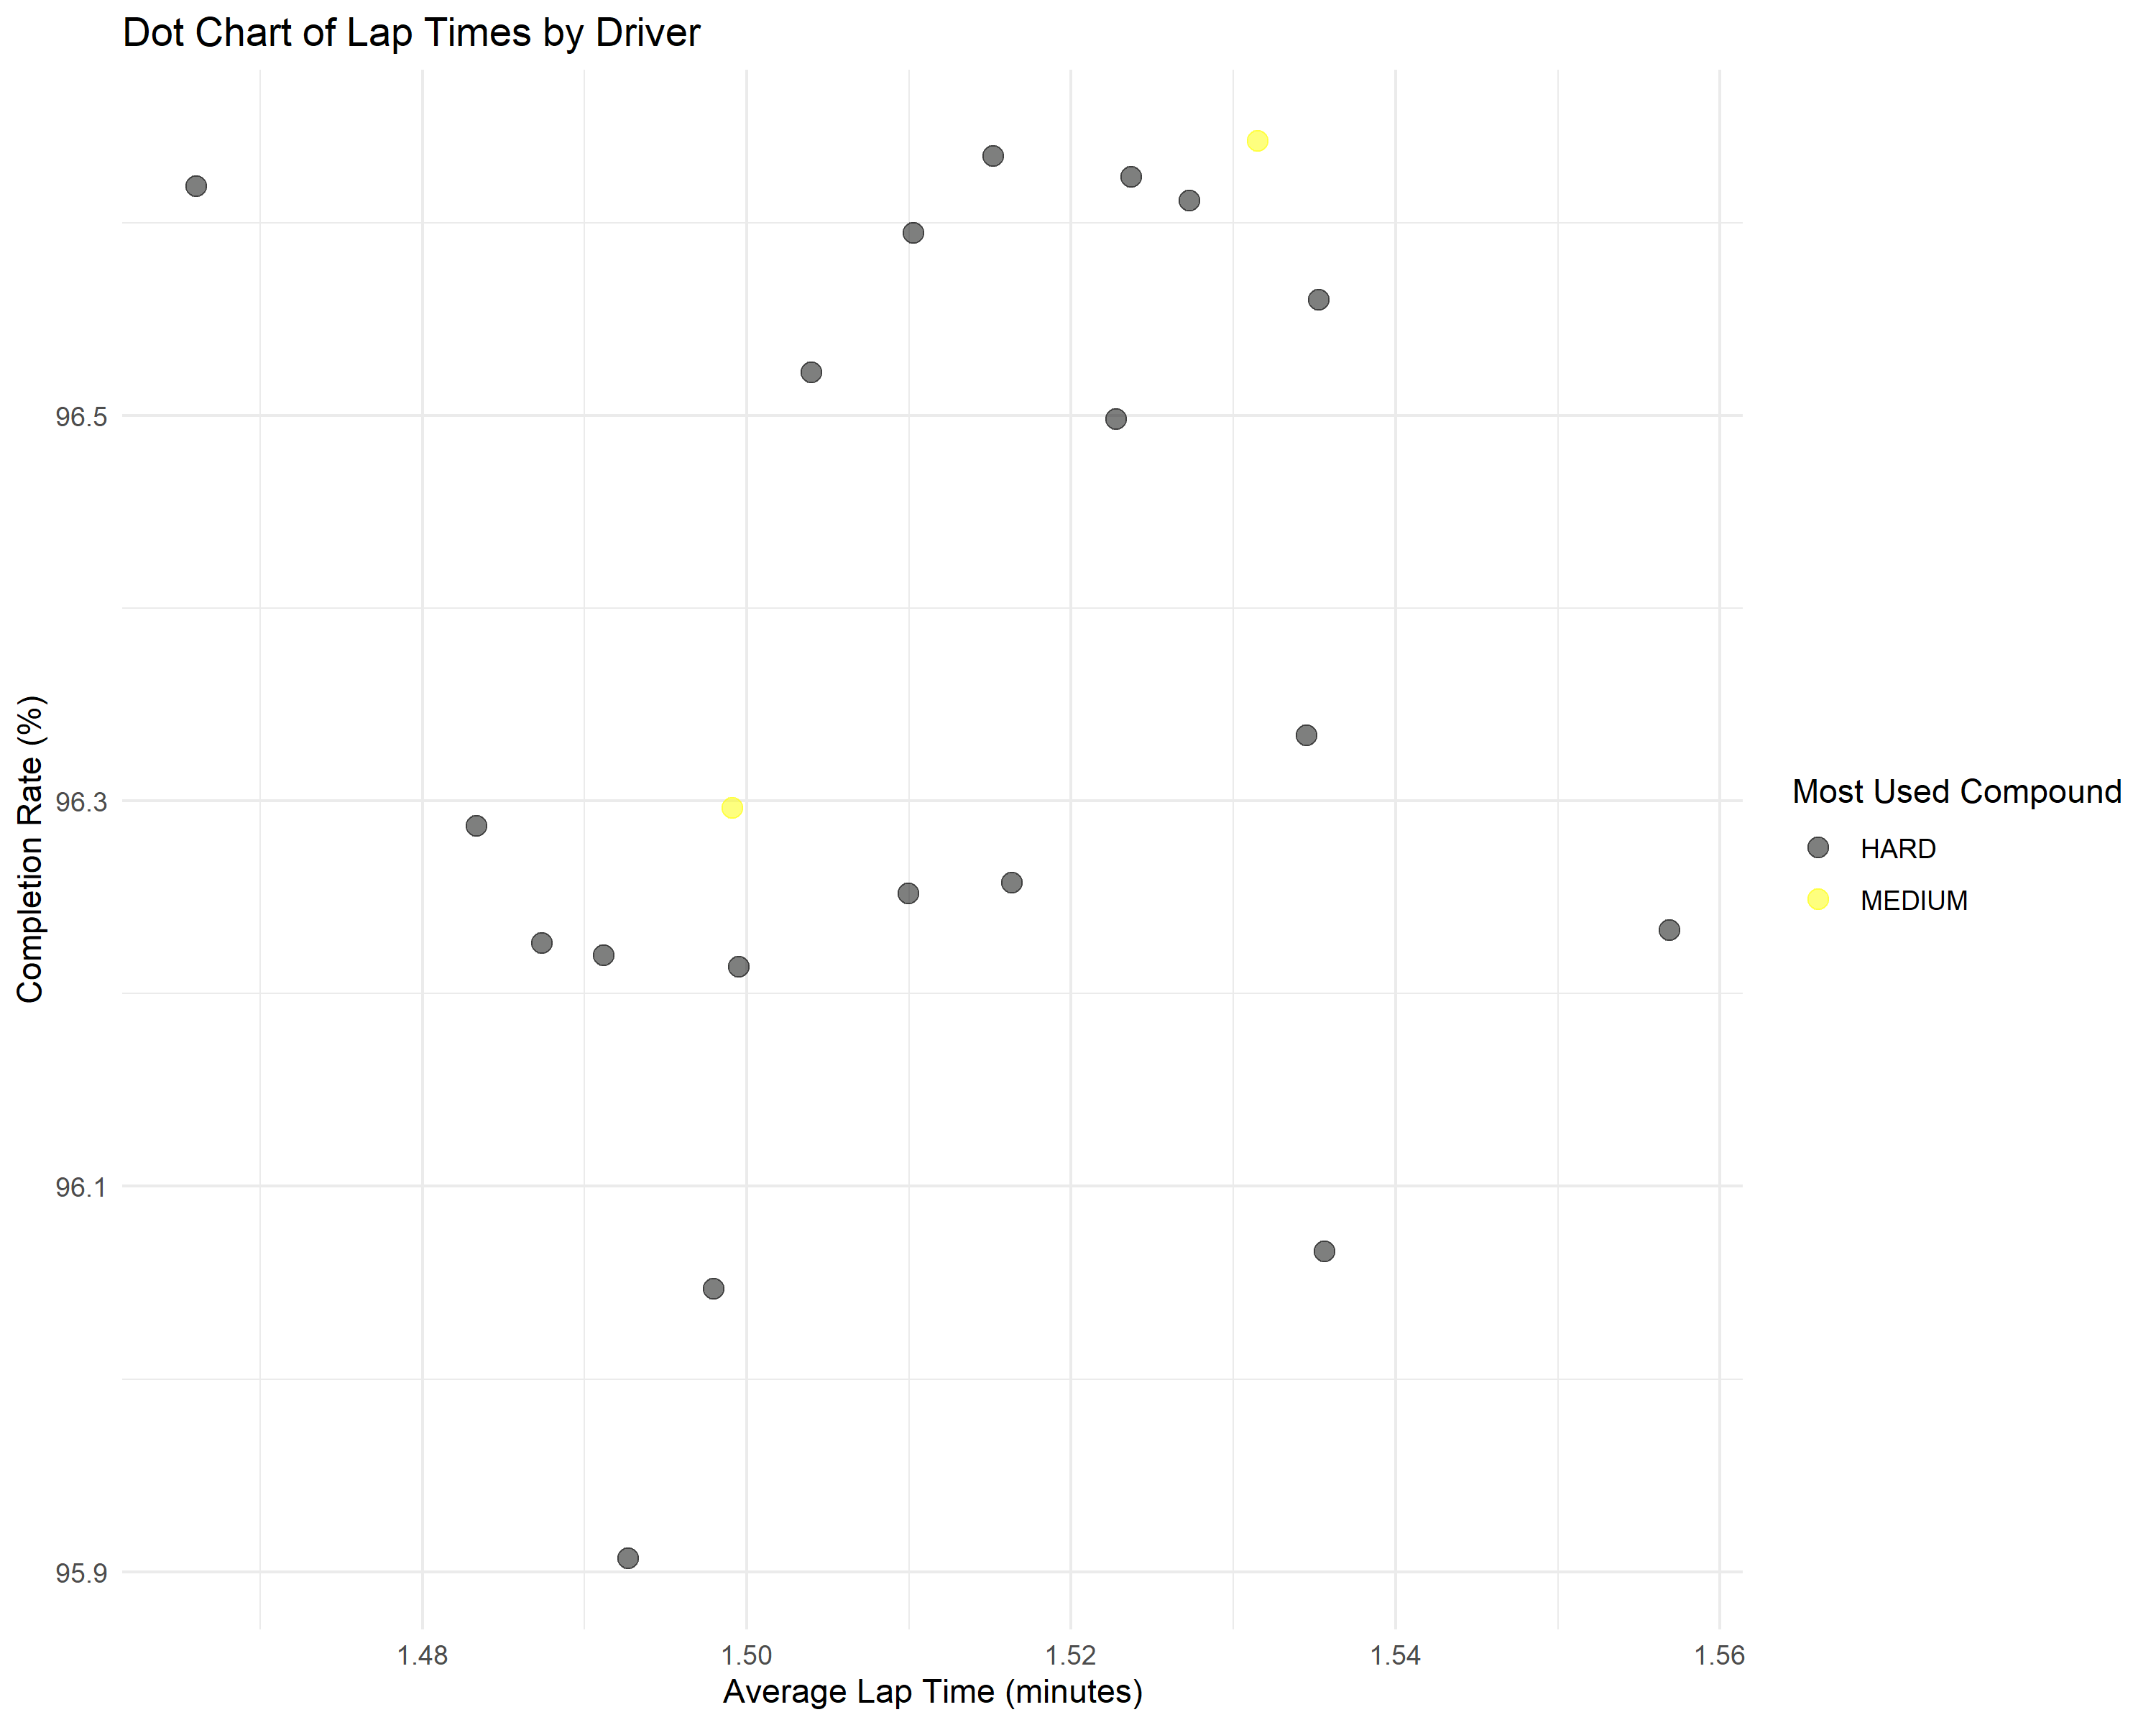
\includegraphics[width=\textwidth]{LapTimesDotChart.png}
    \caption{Dot Chart Overview by Driver}
\end{figure}

\paragraph{Interpretation:}
The dot chart presents a comparison of drivers' average lap times with a color-coded indication of their most utilized tire compound. This visualization can highlight patterns and preferences in tire usage, as well as their impact on lap performance. The completion rate on the y-axis further adds context, indicating reliability or potential issues during races. Together, these metrics allow teams to fine-tune their strategies, particularly around tire selection and management during various phases of a race.

\section{Challenges Encountered}
During the development and analysis phases of our project, we encountered several challenges that fell into two main categories: infrastructure-related and query/code-related. Below, we detail these issues and how we addressed them.

\subsection{Infrastructure-Related Challenges}
\textbf{Google Cloud Storage (GCS) Bucket Naming Error:}
We encountered an error related to the naming of the Google Cloud Storage (GCS) bucket. The error message indicated that the bucket name contained invalid characters, which are restricted in GCS naming conventions.

\begin{enumerate}
    \item \textbf{Bucket Name:} GCS bucket names can only include lowercase letters (a-z), numbers (0-9), underscores (\_), hyphens (-), and dots (.). Spaces and uppercase letters are not permitted. This error stemmed from an oversight in the initial naming phase.
\end{enumerate}

\begin{figure}[H]
    \centering
    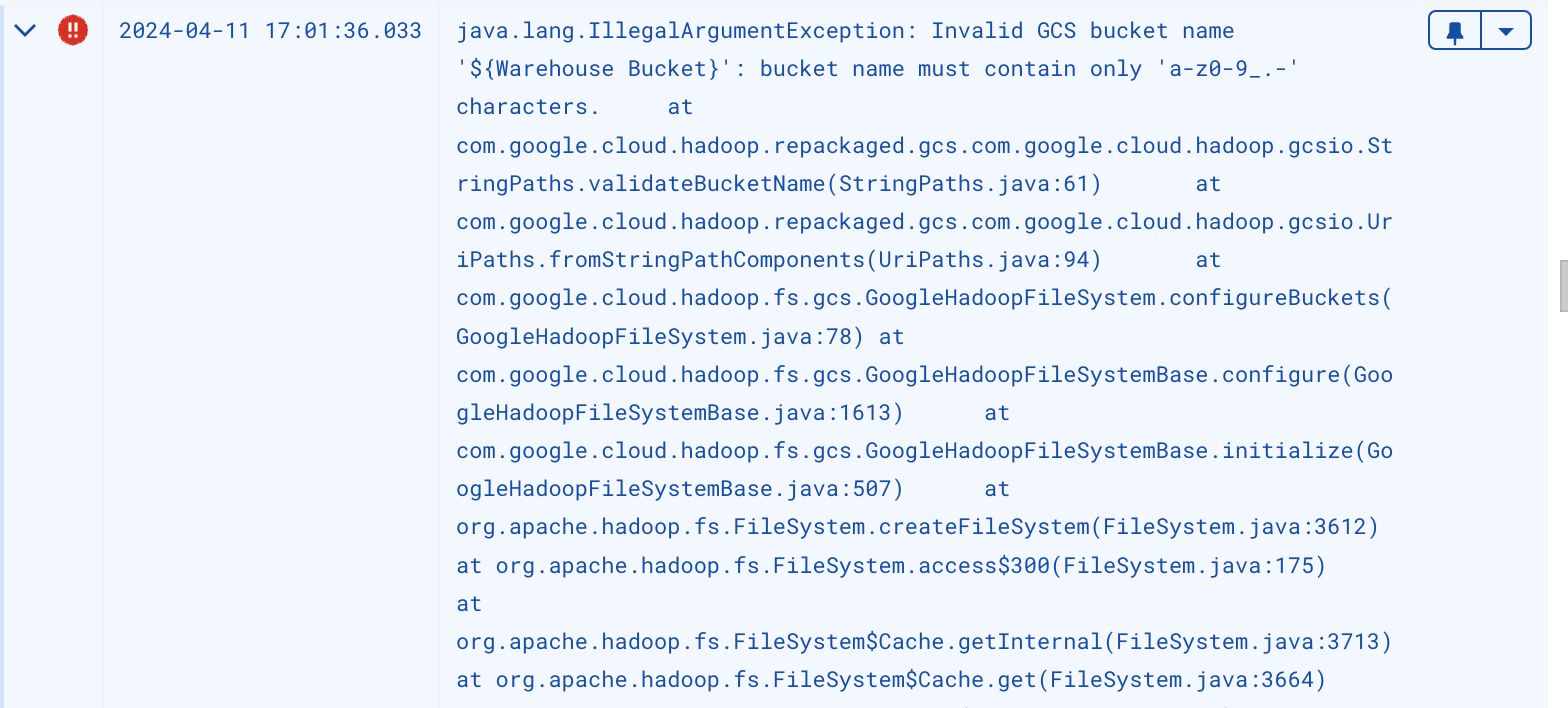
\includegraphics[width=0.9\textwidth]{bucket-name.jpeg}
    \caption{Bucket Name Error}
\end{figure}

To solve this issue, we renamed the bucket to comply with the GCS naming conventions by removing any special characters.

\subsection{Query and Code-Related Challenges}
\textbf{SQL Syntax Errors:}
While executing our SQL queries on the Google Cloud Platform, we faced some errors. These issues were largely due to our initial lack of familiarity with the specific limitations and unique characteristics of SQL functions and data types supported by Google Cloud services. This lack of understanding led to incorrect usage in our queries, impacting our ability to execute them efficiently.

\textbf{Spark SQL AnalysisException:}
In the data processing phase using Spark SQL, we encountered some `AnalysisException` which indicated a misuse of outer query columns in subqueries. Specifically, we faced issues with queries that incorrectly referenced outer columns in subqueries due to the scoping and execution constraints of Spark SQL.

\begin{lstlisting}[language=SQL]
SELECT
    l.Driver,
    (SELECT Compound
     FROM laps
     WHERE Driver = l.Driver AND LapTime IS NOT NULL
     GROUP BY Compound
     ORDER BY COUNT(*) DESC LIMIT 1) AS MostUsedCompound,
    AVG(
        SUBSTRING_INDEX(SUBSTRING_INDEX(LapTime, ' days ', 1), ' days ', -1) * 1440 +
        SUBSTRING_INDEX(SUBSTRING_INDEX(SUBSTRING_INDEX(LapTime, ' days ', -1), ':', 1), ' ', -1) * 60 +
        SUBSTRING_INDEX(SUBSTRING_INDEX(SUBSTRING_INDEX(LapTime, ':', 2), ':', -1), ' ', 1) +
        SUBSTRING_INDEX(SUBSTRING_INDEX(LapTime, ':', -1), '.', 1) / 60
    ) AS AvgLapTime,
    (COUNT(l.LapTime) / COUNT(*)) * 100 AS CompletionRate
FROM
    laps l
GROUP BY
    l.Driver
ORDER BY
    CompletionRate DESC, AvgLapTime;
\end{lstlisting}

\begin{figure}[H]
    \centering
    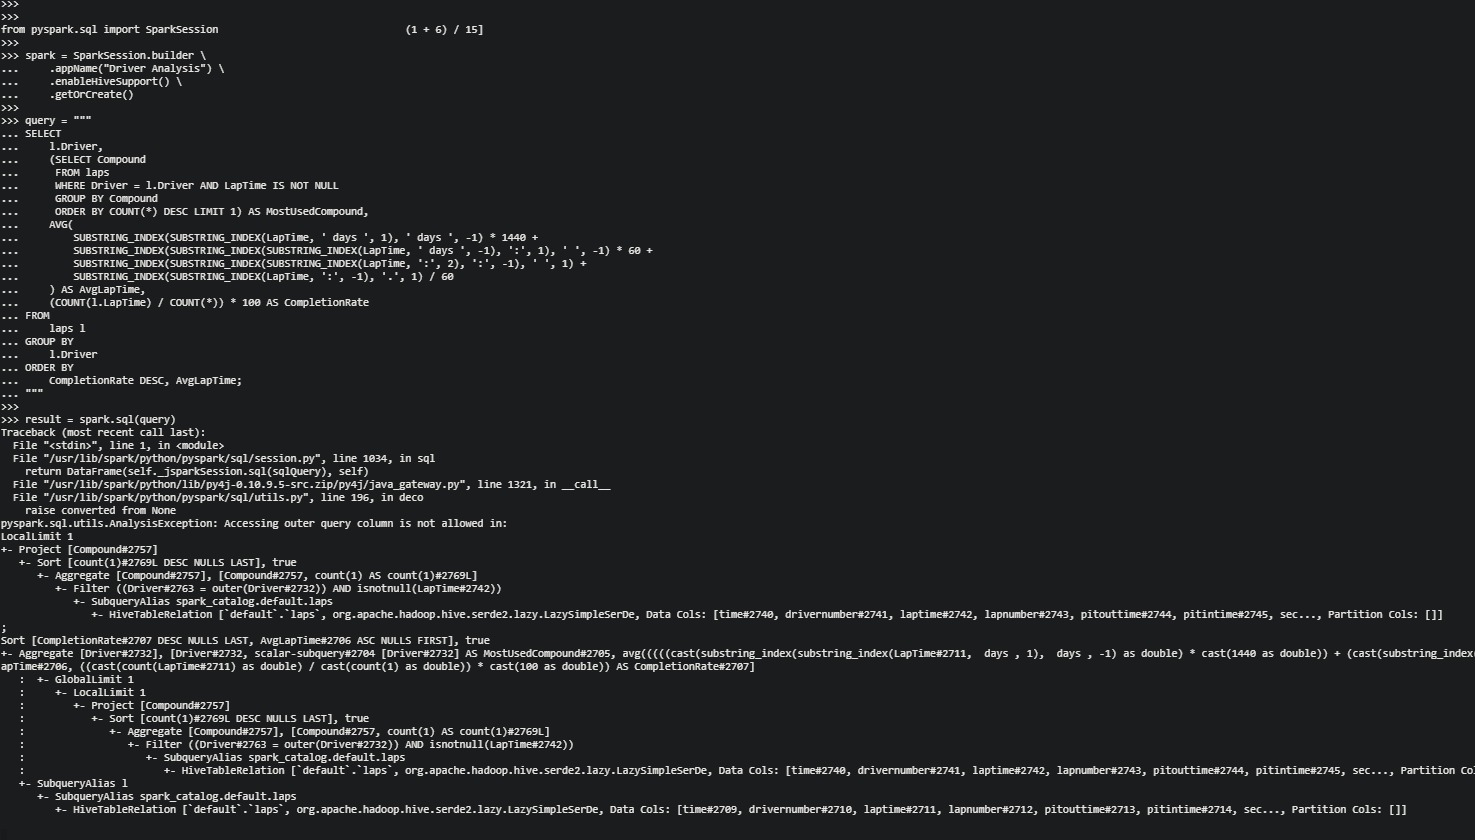
\includegraphics[width=\textwidth]{error-sparkanalysisexception.jpeg}
    \caption{Spark SQL AnalysisException encountered during data processing}
\end{figure}

To address this problem, the SQL query needed to be restructured to avoid direct references to outer query columns within subqueries. Instead of segregating computations, we implemented window functions that allowed us to perform necessary calculations in a single pass of the data. This method retains the context of each row within its partition, enabling us to carry out more complex analyses like ranking and aggregation without resorting to subqueries.

\textbf{Window Functions Implementation:}
The updated code segment utilizes window functions to identify the most used compound by each driver. Following this, we aggregate average lap times and completion rates, all within the same query framework. This approach effectively sidesteps the restrictions imposed by subquery referencing and leverages the powerful analytical capabilities provided by Spark SQL’s window functions:

\begin{lstlisting}[language=Python]
from pyspark.sql import SparkSession
from pyspark.sql.functions import col, expr, count, when, avg
from pyspark.sql.window import Window

spark = SparkSession.builder \
    .appName("Driver Analysis Without Subqueries") \
    .enableHiveSupport() \
    .getOrCreate()

compounds_usage = spark.sql("""
SELECT Driver, Compound, COUNT(*) AS UsageCount
FROM laps
WHERE LapTime IS NOT NULL
GROUP BY Driver, Compound
""")

windowSpec = Window.partitionBy("Driver").orderBy(col("UsageCount").desc())
most_used_compound = compounds_usage.withColumn("rank", row_number().over(windowSpec)) \
    .filter(col("rank") == 1) \
    .drop("UsageCount", "rank")

driver_stats = spark.table("laps_temp").groupBy("Driver").agg(
    avg(
        when(col("LapTime").isNotNull(),
             expr("""
                SUBSTRING_INDEX(SUBSTRING_INDEX(LapTime, ' days ', 1), ' days ', -1) * 1440 +
                SUBSTRING_INDEX(SUBSTRING_INDEX(SUBSTRING_INDEX(LapTime, ' days ', -1), ':', 1), ' ', -1) * 60 +
                SUBSTRING_INDEX(SUBSTRING_INDEX(SUBSTRING_INDEX(LapTime, ':', 2), ':', -1), ' ', 1) +
                SUBSTRING_INDEX(SUBSTRING_INDEX(LapTime, ':', -1), '.', 1) / 60
             """)
        )
    ).alias("AvgLapTime"),
    (count(when(col("LapTime").isNotNull(), 1)).cast("double") / count("*").cast("double") * 100).alias("CompletionRate")
)

final_result = driver_stats.join(most_used_compound, ["Driver"], "left") \
    .select("Driver", "Compound", "AvgLapTime", "CompletionRate") \
    .orderBy(col("CompletionRate").desc(), col("AvgLapTime"))

final_result.show()
\end{lstlisting}

By applying this method, we successfully circumvented the limitation and obtained the required analysis results.

\subsection{Data Integrity Challenges}
\textbf{Handling Nulls as Empty Strings:}
We experienced challenges in calculating accurate percentages in our data analysis due to an unexpected behavior of Google Cloud, which treated null values as empty strings. This discrepancy led to incorrect computation of metrics, affecting the integrity of our results.

\begin{figure}[H]
    \centering
    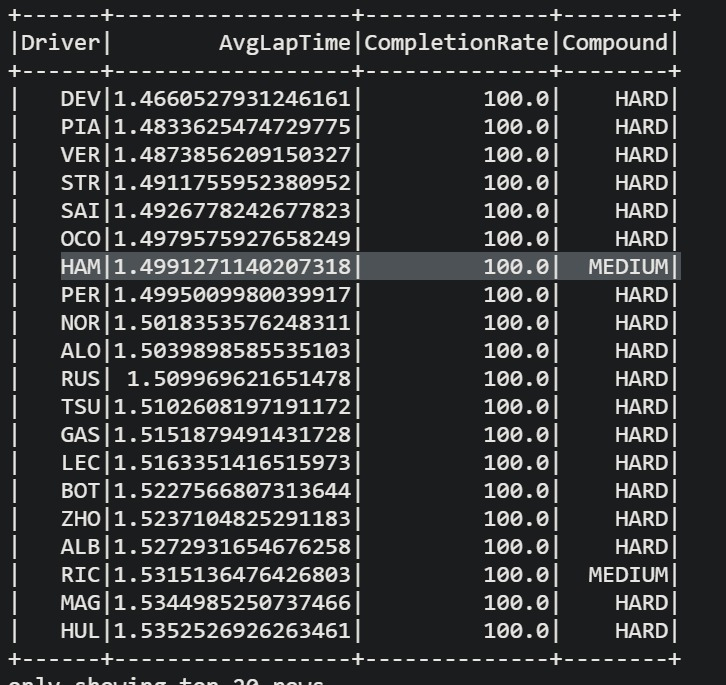
\includegraphics[width=0.6\textwidth]{error-percentages.jpg}
    \caption{Error when calculating Average Lap Time and Completion rate}
\end{figure}


\begin{figure}[H]
    \centering
    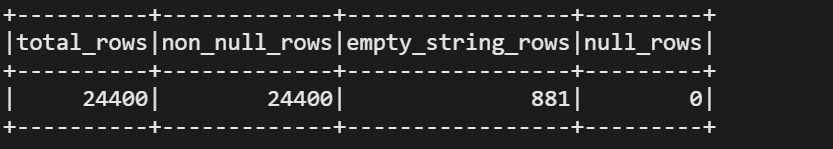
\includegraphics[width=\textwidth]{error-integrity-nulls-empty.jpg}
    \caption{Null and Empty Rows}
\end{figure}

To solve this, we modified our data processing steps using Spark SQL to explicitly replace empty strings with null values, ensuring the accuracy of subsequent computations. The following code snippet shows the adjustments made to the `LapTime` data:

\begin{lstlisting}[language=Python]
from pyspark.sql import SparkSession
from pyspark.sql.functions import col, when

spark = SparkSession.builder
    .appName("Update LapTimes")
    .enableHiveSupport()
    .getOrCreate()

laps_df = spark.table("laps")

laps_df_updated = laps_df.withColumn(
    "LapTime",
    when(col("LapTime") != "", col("LapTime")).otherwise(None)
)

laps_df_updated.createOrReplaceTempView("laps_temp")

result = spark.sql("""
    SELECT Driver, COUNT(*) AS TotalLaps, SUM(CASE WHEN LapTime IS NULL THEN 1 ELSE 0 END) AS NullLapTimes
    FROM laps_temp
    GROUP BY Driver
""")

result.show()
\end{lstlisting}

The corrected calculations revealed the true distribution of null values, which is essential for accurate data analysis. This adjustment was a critical step in maintaining the quality and reliability of our data-driven insights.

\begin{figure}[H]
    \centering
    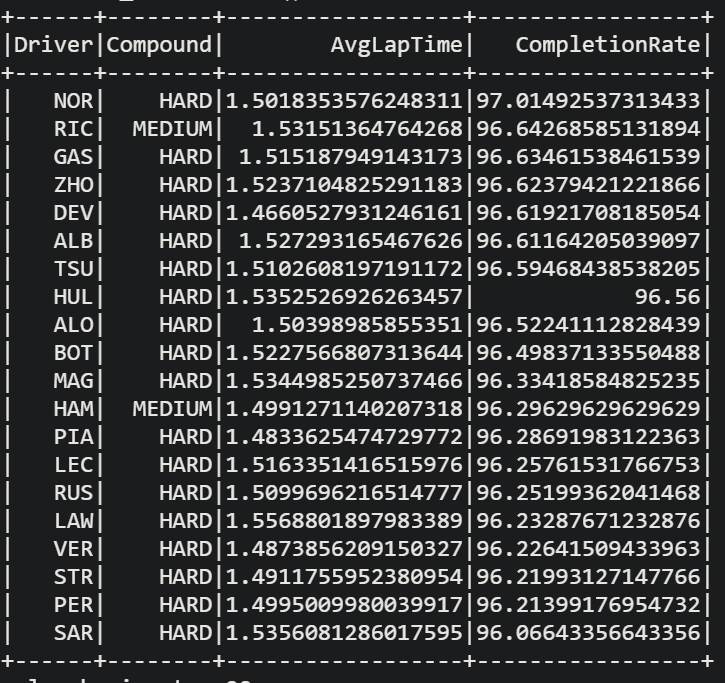
\includegraphics[width=0.6\textwidth]{solved-nulls.png}
    \caption{Final Result With Accurate Null Lap Times}
\end{figure}


Each challenge was carefully addressed to ensure continuation of our project, allowing us to leverage full capabilities of our big data infrastructure and analytical tools.

\section{Data Processing Optimizations}
\subsection{Conversion of Lap Times for Simplified Access}
During our analysis, we recognized the need for a standardized format for lap times to facilitate easier access and more efficient queries. To achieve this, we created a user-defined function (UDF) that converts the lap times into a consistent unit of minutes, thus normalizing the data and making subsequent analyses more straightforward.

\textbf{Lap Time Conversion:}
The code snippet below details the UDF convert\_laptime\_to\_minutes that we applied to the entire dataset. This function parses the original lap time strings and calculates the total time in minutes, which is then used to update the dataset. The resulting table, laps\_temp\_updated, provides a clean, uniform set of lap times across all entries, significantly optimizing our data processing pipeline:

\begin{lstlisting}[language=Python]
from pyspark.sql import SparkSession

spark = SparkSession.builder \
    .appName("Weather Insights") \
    .enableHiveSupport() \
    .getOrCreate()

weather_insights_query = """
SELECT
    EventName,
    Compound,
    AVG(LapTime) AS AvgLapTime,
    TemperatureCondition,
    HumidityCondition
FROM (
    SELECT
        l.EventName,
        l.Compound,
        l.LapTime,
        CASE
            WHEN AVG(w.AirTemp) OVER (PARTITION BY l.EventName) >= 25 THEN 'Hot'
            WHEN AVG(w.AirTemp) OVER (PARTITION BY l.EventName) BETWEEN 15 AND 24 THEN 'Mild'
            ELSE 'Cold'
        END AS TemperatureCondition,
        CASE
            WHEN AVG(w.Humidity) OVER (PARTITION BY l.EventName) > 70 THEN 'High Humidity'
            ELSE 'Low/Medium Humidity'
        END AS HumidityCondition
    FROM
        laps_temp_updated l
    JOIN
        weather w ON l.EventName = w.EventName
    WHERE
        l.LapTime IS NOT NULL  
) sub
GROUP BY
    EventName, Compound, TemperatureCondition, HumidityCondition
ORDER BY
    EventName, AvgLapTime;
"""

weather_insights = spark.sql(weather_insights_query)
weather_insights.show()

\end{lstlisting}
This transformation has streamlined our data handling, making it much more efficient for subsequent SQL queries to perform analyses, such as calculating weather insights or identifying best times in each Grand Prix. By normalizing the lap times, we have reduced the complexity and potential for errors in our data-driven insights.



\section{Hive Metastore}
\subsubsection{SQL Connection to the Hive Metastore with the SDK}
\begin{lstlisting}[language=bash]
cloud sql connect formula1-bigdata-term2-up-sql --user=root
\end{lstlisting}

\subsubsection{Selecting Database}
Once the connection is established, we select the \textit{hive\_metastore} database to perform operations on the metastore tables.

\begin{lstlisting}[language=SQL]
USE hive_metastore;
\end{lstlisting}

\subsubsection{Querying the Table Location}
The following query is designed to retrieve metadata from the Hive Metastore regarding the storage details of a specific table. In this case, the table in question is `laps`. 

\begin{lstlisting}[language=SQL]
SELECT s.* FROM `hive_metastore`.`TBLS` t
JOIN `hive_metastore`.`DBS` d ON t.`DB_ID` = d.`DB_ID`
JOIN `hive_metastore`.`SDS` s ON t.`SD_ID` = s.`SD_ID`
WHERE t.`TBL_NAME` = 'laps' AND d.`name` = 'default';
\end{lstlisting}

This query joins three critical tables of the Hive Metastore:
\begin{itemize}
    \item \texttt{TBLS} - Contains metadata about the tables including the table name and associated database and storage descriptors.
    \item \texttt{DBS} - Stores details about databases such as names and descriptions.
    \item \texttt{SDS} - Holds storage descriptors which include information about the physical storage of the data (such as location, input/output format, etc.).
\end{itemize}

\begin{figure}[H]
    \centering
    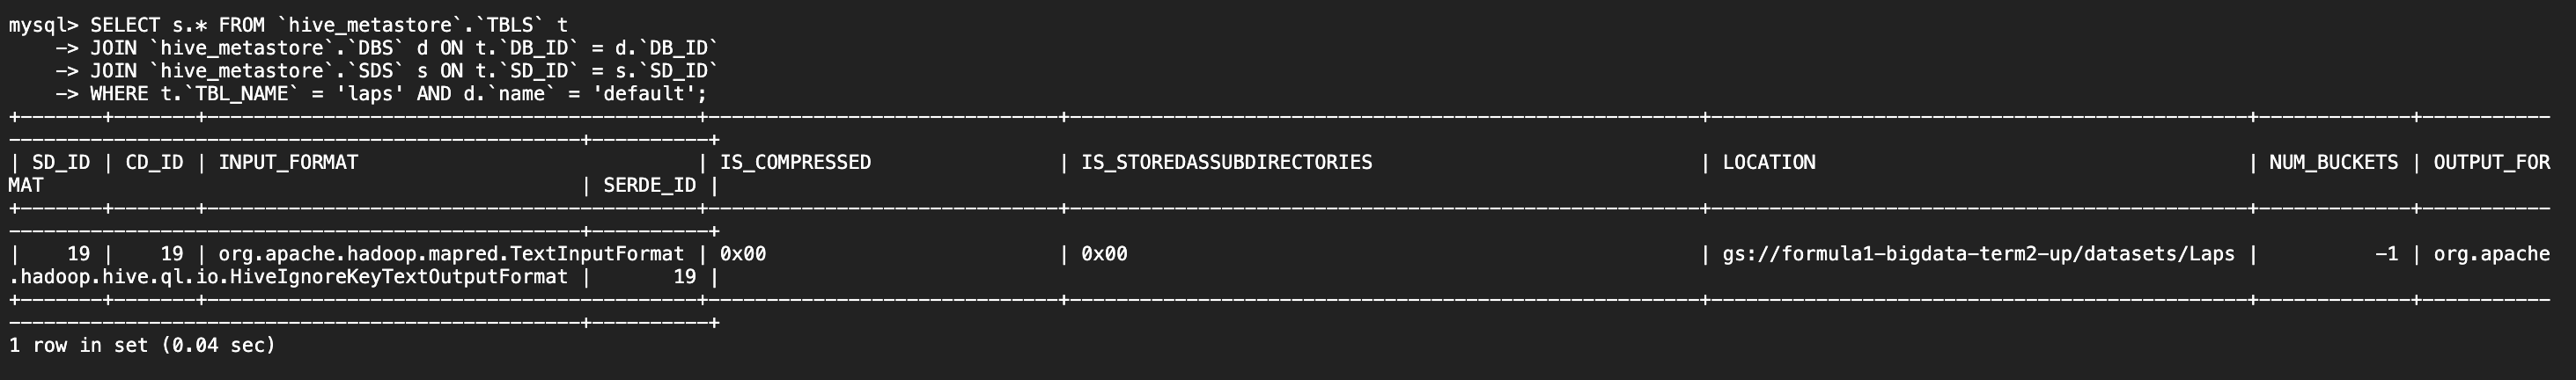
\includegraphics[width=\textwidth]{hive1.png}
    \caption{Searching Data Location}
\end{figure}

\subsubsection{Querying Data Format and Location}
The SQL command below is utilized to fetch the data input format and the storage location of the `Laps` table. This query is crucial for understanding how the data is read and where it is physically stored.

\begin{lstlisting}[language=SQL]
SELECT INPUT_FORMAT, LOCATION
FROM SDS s, TBLS t
WHERE s.SD_ID = t.SD_ID AND t.TBL_NAME = 'Laps';
\end{lstlisting}

The query performs a simple join between the `SDS` (Storage Descriptors) table and the `TBLS` (Tables) table on the `SD\_ID` field, which links the table's storage information to its physical metadata. The `INPUT\_FORMAT` field provides insight into the data serialization and deserialization format, and the `LOCATION` field specifies the exact path in the storage system where the table's data files reside.

\begin{figure}[H]
    \centering
    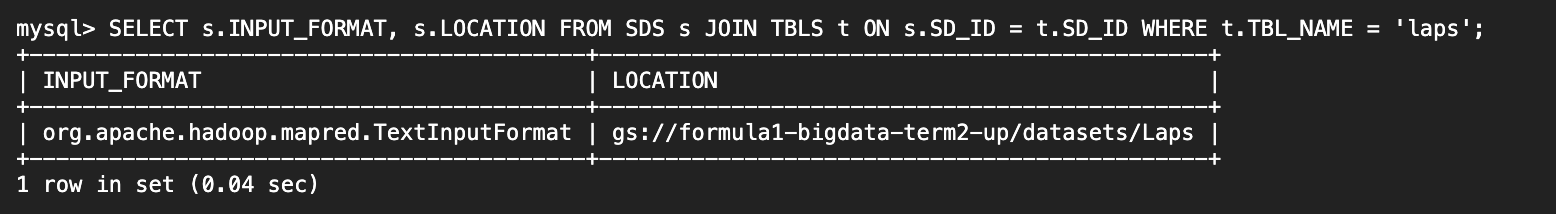
\includegraphics[width=\textwidth]{hive2.png}
    \caption{Searching Data Format}
\end{figure}


\section{Conclusions}
Through the utilization of big data technologies such as Hadoop and Hive on the Google Cloud Platform, this project has provided significant insights into the 2023 Formula 1 season. Our comprehensive analysis spanned multiple aspects of the sport, from individual driver performance and tire strategies to the influence of weather conditions on race dynamics.

\paragraph{Insights and Impact:}
The queries conducted revealed:
\begin{itemize}
    \item The average number of laps per Grand Prix can inform race strategies and pit stop planning.
    \item Tire compound usage rates can help teams optimize tire strategies for different tracks and conditions.
    \item The density of drivers per event can influence the competitiveness and excitement of a race.
    \item Driver lap completion rates are crucial for assessing reliability and potential technical issues.
    \item Telemetry data provides a deep dive into driving styles and can influence car setup and driver training.
\end{itemize}

Furthermore, the challenges faced during the project, such as data integrity issues and the necessity for query optimization, were successfully overcome. These solutions not only enhanced the accuracy of our analysis but also enriched our understanding of the capabilities and limitations of the tools used.

\paragraph{Future Directions:}
Our project serves as a testament to the potential of big data in sports analytics. The methodologies and processes established here can be extended to other sports disciplines. There's an opportunity to integrate real-time data analysis for dynamic strategic decision-making during races. Additionally, machine learning could be employed to predict outcomes based on historical and live data streams, providing an even richer set of insights for teams and fans alike.

\paragraph{Final Thoughts:}
The intersection of big data and sports represents a fertile ground for innovation. This project has not only contributed to the field of sports analytics but also demonstrated the practical applications of big data technologies in real-world scenarios. The findings can aid teams in making data-driven decisions that refine performance and strategies, ultimately elevating the sporting spectacle of Formula 1 racing.

As the technology landscape evolves, so too will the capabilities for data analysis within the sport. We look forward to seeing how future developments will continue to transform the way teams and fans engage with Formula 1.

\section{Project Repository}
\url{https://github.com/enriquegomeztagle/BigData/tree/main/SecondTerm/F1-EDA-Project}

\section{References}
\label{sec:references}
\begin{enumerate}
    \item Hadoop: \url{https://hadoop.apache.org/}
    \item Hive: \url{https://hive.apache.org/}
    \item Cloud SQL: \url{https://cloud.google.com/sql}
\end{enumerate}

\end{document}
